%%%%%%%%%%%%%%%%%%%%%%%%%%%%%%%%%%%%%%%%%
% University/School Laboratory Report
% LaTeX Template
% Version 3.1 (25/3/14)
%
% This template has been downloaded from:
% http://www.LaTeXTemplates.com
%
% Original author:
% Linux and Unix Users Group at Virginia Tech Wiki 
% (https://vtluug.org/wiki/Example_LaTeX_chem_lab_report)
%
% License:
% CC BY-NC-SA 3.0 (http://creativecommons.org/licenses/by-nc-sa/3.0/)
%
%%%%%%%%%%%%%%%%%%%%%%%%%%%%%%%%%%%%%%%%%

%----------------------------------------------------------------------------------------
%	PACKAGES AND DOCUMENT CONFIGURATIONS
%----------------------------------------------------------------------------------------

\documentclass{report} %report

\usepackage[version=3]{mhchem} % Package for chemical equation typesetting
\usepackage{siunitx} % Provides the \SI{}{} and \si{} command for typesetting SI units
\usepackage{graphicx} % Required for the inclusion of images
\usepackage{hyperref}
\usepackage{caption}
\usepackage{amsmath} % Required for some math elements 
\usepackage{indentfirst}
\usepackage{dirtytalk}
\usepackage{titlesec}
\usepackage{float}
\usepackage{verbatim}
\usepackage{listings}

\lstset{
  breaklines=true,
}


\title{Enhancing Hearthstone deck building with a Generative Adversarial Network (GAN)} % Title
\titleformat{\chapter}{\normalfont\LARGE\bfseries}{\thechapter.}{18pt}{\LARGE\bfseries}
\titleformat*{\subsection}{\large}
\titleformat*{\subsubsection}{\normalfont}
\author{Callum \textsc{Roberts}} % Author name
\setcounter{secnumdepth}{4}


\renewcommand{\labelenumi}{\alph{enumi}.} % Make numbering in the enumerate environment by letter rather than number (e.g. section 6)
\bibliographystyle{IEEEtran}
%\usepackage{times} % Uncomment to use the Times New Roman font

%----------------------------------------------------------------------------------------
%	DOCUMENT INFORMATION
%----------------------------------------------------------------------------------------


\author{Callum \textsc{Roberts}} % Author name

\date{\today} % Date for the report

\begin{document}

\maketitle % Insert the title, author and date

% If you wish to include an abstract, uncomment the lines below
% \begin{abstract}
% Abstract text
% \end{abstract}

%----------------------------------------------------------------------------------------
%	SECTION 1
%----------------------------------------------------------------------------------------
\begin{abstract}

\end{abstract}

\section*{Acknowledgements}
I would like to thank, in particular, my project supervisor Mark Bartlett, whose wisdom proved invaluable to the completion of this project. This thanks extends to the rest of the RGU staff who went beyond expectations in their support during these tough times.

Thanks are also owed to the Hearthpwn team who allowed me to collect their data and to the HearthSim team for their simulator to run the tests.


\tableofcontents

\chapter{Introduction}
\section{Overview}
Bringing Artificial Intelligence to Hearthstone: Heroes of Warcraft is not a new concept, it has been subject to many studies in the field, where it be playing the game, suggesting moves to the player or building decks. Focusing on the field of deck building, it is a concept that exists across multiple trading card games such as Magic: The Gathering, Pokemon, Yu-Gi-Oh! and of course Hearthstone. Papers have studied these games more or less, but all seem to gravitate around similar deck building techniques, details of which will be expanded later on. These techniques seemingly been saturated, newer studies apply small scale changes to already defined methods \cite{Back1996}. Exploration of different techniques has been touched on but they seem to be outliers and of limited number \cite{Ward2020}, experimenting with other algorithms could show better, more  interesting results instead of assuming that one saturated method is the best because of its popular usage.
\section{Motivation}
Using a Artificial Intelligence algorithm that has not been utilised nor researched in the field of deck building could provide insight into the Generative Adversarial Network (GAN) applications in other fields of research, as it is mostly limited to image generation. Along with this discovering another method for deck building that could bear fruit to similar or improved results, opening the way for more techniques and deeper research into the use of recorded data for deck generation. 
\section{Aims and Objectives}
The aim of this project is to create a deck building artificial intelligence using a Generative Adversarial Network (GAN) and testing the viability of it, this will be achieved by completing the following objectives:
\begin{itemize}
  \item Collecting user deck data from reliable sources
  \item Cleansing of user deck data
  \item Converting user deck data to vectors and back to human readable after training
  \item Implement GAN for single dimensional vector generation
  \item GAN hyper-parameter and layer optimization
  \item Simulating results against user decks
  \item Performing evaluations on resulting decks
\end{itemize}
\section{Key Findings}
This project has exhibited that it is possible to use Generative Adversarial Networks to generate decks for Hearthstone, a technique that seemingly no one has attempted to use, the AI demonstrates similarities to user created decks such as card types, type percentage, card duplicates, synergies and card spread. The decks tested have an average of 55\% win rate, varying from class to class, match ups against other classes greatly influenced the outcome of a match. Although the win rate is heavily influenced by the AI playing it, considering that the simulator game playing AI will not play as well as a human player. The training process is much faster than anticipated (around 10 minutes), however the testing was much longer at around 1 - 2 hours depending of the number of decks created.
\section{Structure}
The structure of the report is as follows, first a literature review which presents an overview of Hearthstone, some of the important game mechanics and existing AI that have been used. Then a discussion  of  the  requirements  of  the  project  and  the  methodology  to implement them. Following this is a discussion of the potential legal and ethical issues with the project and what has been done to overcome them. The implementation of the project, a deep dive into how the project was completed. A testing and evaluation section describing the strategy and the results of the generated decks. Finally, a conclusion which summarises the project is given.

\chapter{Literature Review}
The purpose of this literature review is to define the technologies used in the field of artificial intelligence for building a deck in Hearthstone. To introduce, and compare previous works to determine their strengths and weaknesses. A review of the literature is valuable in understanding important aspects of a research area \cite{Isaacs2020}. The structure of this literature review is as follows: the initial section will detail the background of the project, explaining the fundamentals of Hearthstone and deck building. Following that will be an introduction to the project,  motivations, and research questions. Finally, we will have the core technologies used for similar projects.
\section{Background}
	For the benefit of the reader, this section will introduce the basics of Hearthstone. It will emphasize the deck building aspect of the game including practices used by players.  
\subsection{Collectible Card Games}
	Collectible Card Games (CCG)\footnote{\url{https://en.wikipedia.org/wiki/Collectible_card_game}} are a sub-genre of card games introduced in 1993 by Magic: The Gathering \footnote{\url{https://en.wikipedia.org/wiki/Magic:_The_Gathering}}. They require players to make a custom decks to play, they mix trading cards with strategy and deck building features. CCGs are usually defined as a turn-based game, where each player acquires their own collection of cards through the purchasing of "starter decks" for beginners or "booster packs" containing a small number of random cards from a {\it{pool}} of cards usually referred to as an expansion. The aim is to build an efficient deck that can account for the inconsistency that comes from the nature of card games, to predict and play around your opponent's actions to ultimately beat them. Some CCGs can prove to be lucrative for players as cards have a value intrinsic to their rarity and demand \footnote{\url{https://www.cardmarket.com/en/Magic/}}, this makes building the perfect deck rather difficult and usually costly.
\subsection{Hearthstone}
	Hearthstone: Heroes of Warcraft is a CCG developed by Blizzard Entertainment in 2013 \cite{HS}, but with the twist of it being entirely digital, there is no physical version of the game. This choice unlocks potential for gameplay features that could not be implemented, in exchange for the tradability of cards. \\ 
\begin{figure}[h]
\centering
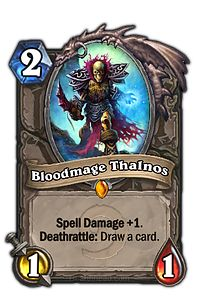
\includegraphics[width=0.25\textwidth]{thalnos}
\caption{Example of a Legendary Hearthstone card\protect\footnotemark
\label{card}
}
\end{figure}
\footnotetext{\url{https://www.pinterest.fr/pin/573716440004576557/}}

	\indent Two players face off wielding each a deck of their own making. Decks consist of exactly 30 cards. Players then take it in turns to play their cards, the objective being to reduce the other player's health to zero. On each player's turns that player draws a card and gains a “Mana Crystal” up to a maximum of 10 (crystals are refreshed every turn), these crystals are expended to cast a card from the player's hand. Before a match each player chooses to embody a class (such as Mage, Warrior, Rogue, Druid, etc…), each class has specific cards only they can add into their deck, these are adequately named “Class Cards”, these are accompanied by “Neutral Cards” that any class can use. Classes also have access to an ability unique to them called a "hero power". \\
	
\begin{figure}[h]
\centering
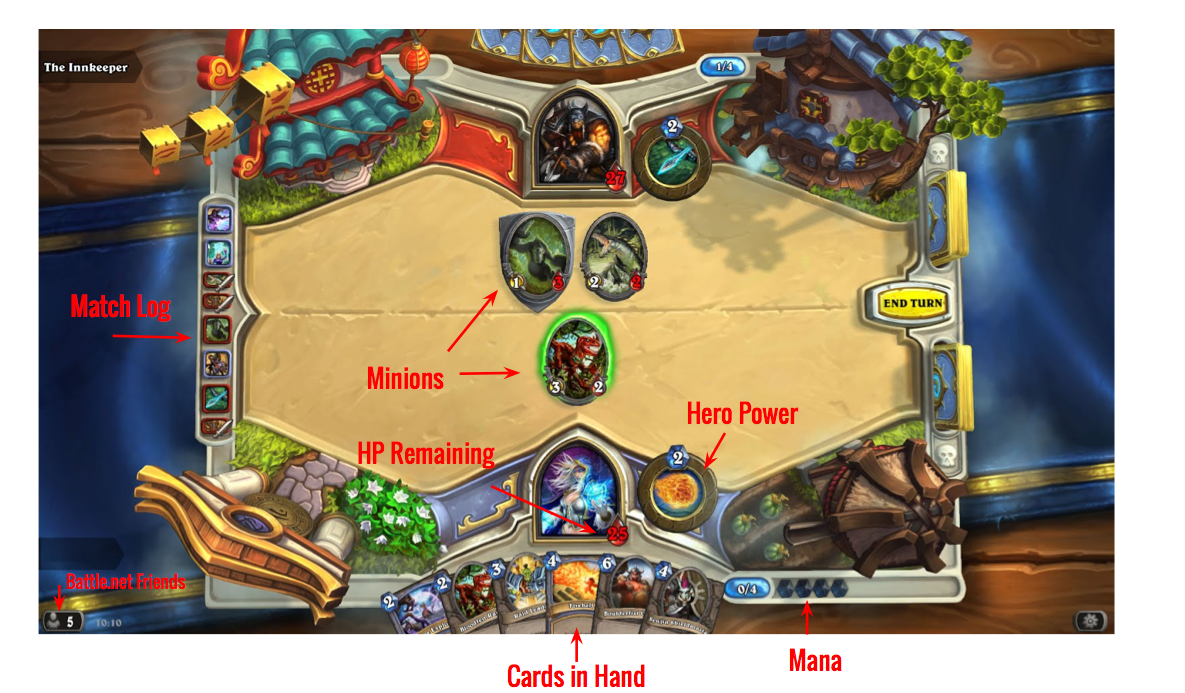
\includegraphics[width=1\textwidth]{hearthstonegameboard}
\caption{Example of a Hearthstone board\protect\footnotemark}
 \label{board}
\end{figure}
\footnotetext{\url{https://bothgunsblazingblog.wordpress.com/2014/06/22/hearthstone-analysis-and-deconstruction/}}
	
	Each card in the game has a “mana” cost which shows how many mana crystals are needed to cast that card. They also have a card type, rarity, and an effect. In a deck, players can put duplicates of the same card (up to 2) except for "Legendary Cards" (figure \ref{card}) that are limited to a single copy due to their powerful effects.  Players have a “Collection”, where the cards they own are stored, to get new cards players can buy card packs with gold, the in-game currency of Hearthstone. Gold is earned slowly through quests, winning, and events, however this process can be sped up through the purchase of gold with real-life currency. Players can also choose to "Disenchant" their duplicate cards to gain another in-game currency called "Dust" which can be used to create a card of the players choosing\footnote{\url{https://hearthstone.gamepedia.com/Crafting}}.


\subsection{Deck Building}
	In the world of CCGs, there is a long-standing debate on how to measure the skill of a player. Although card games involve luck and circumstance, it is believed that there is a degree of strategy in the building and execution of decks whether it is just a slight increase in win probability or a fundamental to winning \cite{SvsL}. However, the debate stems from which is the most important, the building aspect or the execution aspect of CCGs.
	\cite{BvsP}
	\subsubsection{Metagame}
	Hearthstone is a game with lots of complex systems that are influenced by many factors, mainly due to a large number of cards and different playable heroes. In a game where there are lots of variables, players try to rank cards, heroes, and combinations to increase their chances to win. This phenomenon creates decks from a "pool" of top-rated cards, leaving out the mediocre, forcing players to use these top-rated decks in order to have a better chance of winning or be put at a disadvantage. The result is what is called the "Metagame" or {\it{meta}} for short\footnote{\url{https://www.hearthstonetopdecks.com/hearthstones-best-standard-ladder-decks/}}. Blizzard release updates to the game frequently through "expansions"\footnote{\url{https://hearthstone.gamepedia.com/Expansion}} which add a variety of new cards to keep the game fresh. Shifts in the meta occur when these expansions are added and players experiment to find better combinations over time. However better cards may not be added, and changes in the meta may not occur, this dissuades players from continuing or returning to play knowing that they have already experienced all that they can. To avoid that Hearthstone has implemented two-game modes\footnote{\url{https://hearthstone.gamepedia.com/Game_format}}, one in which only cards added over the past two years are available, and another mode that allows all cards. Whilst this method has helped, it still does not put a stop to the possibility of a stale meta. Researchers have done studies on how to evolve the meta through AI means, by {\it{balancing}} powerful cards ({Fernando et al.}) \cite{EvolveMeta}. Balancing a card means to adjust the power of said card to make it more or less viable in the current game environment. Fernando et al. discussed the idea that around 50\% of Hearthstone's meta is derived from match-ups which is the win probability two decks have against each other, a favorable match-up being the one with the highest win probability or known in the community as {\it{win rate}}.  
\subsubsection{Mana Curve}
	Theorycrafting is a term used widely in many video games, it designates a mathematical analysis of a game's core mechanics to attempt to discover new strategies or combinations that could rival the current ones. Hearthstone is one such game, a large portion of the player base enjoys theorycrafting new decks that may {\it{break}} the meta, as in cause a fundamental shift of the current metagame. These players rely on fundamentals or schematics that are used as a guideline in building a new deck. The {\it{mana curve}} \footnote{\url{http://hearthstone.gamepedia.com/Mana_curve}} is one such fundamental, it exists in all decks built in the game. Every card in Hearthstone has a cost, this cost determines the power of the card, a low-cost card will be weaker than a higher cost card since it would cost fewer resources to cast. This {\it{mana curve}} is a histogram of each card plotted by cost, it allows players to visualize how expensive in resources their deck is and to determine the deck's archetype. 
\begin{figure}[h]
\centering
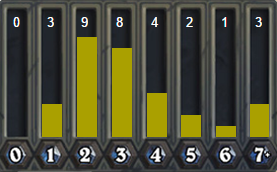
\includegraphics[width=0.5\textwidth]{mana_curve}
\caption{Example of a Mana Curve\protect\footnotemark}
\label{board}
\end{figure}
\footnotetext{\url{https://hearthstone.judgehype.com/deck-mage-tempo-ladder-legendaire-tgt-gvg/}}
\subsubsection{Archetype}
\label{archetypes}
	The word archetype is derived from the Greek word {\it{archétypon}} which means "beginning, origin", applied in the psychology field to categorize complex human behaviour called "Jungian Archetypes" \cite{Robertson2016}. This term was transposed into the deck building field of CCGs, a deck's archetype is meant to categorize and describe the behaviour of the deck from a high-level perspective, forgoing the need to play the deck to learn its strategy. In Hearthstone, most decks can be categorized by three main archetypes \cite{Judlick}:
\begin{itemize}

\item \textit{Aggro} decks are the aggressive decks meant to defeat an opponent as quickly as possible, as a consequence the mana curve of such decks is focused towards the cheaper side of the histogram. Their power comes in the early turns, but they quickly become weaker to the other archetypes as the turns go on.
\item \textit{Control} decks are meant to control the state of the board through the use of expensive cards, they tend to generate a lot of cards and have a wide range of card choices. The mana curve of such an archetype is towards the expensive end of the histogram. They tend to have a few cards to play early in the game but have a multitude of win conditions in later turns.

\item \textit{Mid-range} decks are situated in the middle of the two other archetypes, focusing mainly on the mid-game, their win conditions are stronger than the aggro decks but weaker than the control decks. Their mana curve peaks in the middle of the histogram.
\end{itemize}

Hearthstone also has other archetypes that cover a shorter scale, they are usually introduced in the newer expansions and rotate out of the normal game after a couple of years \cite{Standard}. For example, a highlander archetype is a deck with 30 unique cards. Archetypes are formed around specific cards with win conditions\footnote{\url{https://playhearthstone.com/en-us/news/21363038}}, meaning that they have the power to win the game. So in the example given in a highlander deck, there would be a card that has an effect that triggers from having only unique copies in the deck.
 
\subsubsection{Resource Cost}
	In CCGs, cards have a certain cost to use, in Hearthstone that cost is mana which regenerates every turn. The cost of a card is determined by the power of said card, if it has a powerful effect, has decent attack and defence values, or even both. This cost will determine how late into the game a card can be played. However, a card that costs a lot can be considered weak and a low-cost card can be considered strong. The power of a card is determined through the resource cost, an invisible value that is hard to calculate and a subject of study \cite{Zuin2019}. Although the Zuin et al. study was used to predict the cost of a card in Magic: The Gathering, the resource calculation is still present in Hearthstone. It poses a good solution to the balancing of the metagame and would be adaptable to Hearthstone. A card is considered efficient if the theoretical resource cost is higher than the current mana cost, and would be inefficient if the resource cost were to be lower than the mana cost. The resource cost of a card is something that may need to be considered when developing an AI for building decks. Stiegler et al. \cite{Stiegler2017} applied a similar theory to design a deck-building AI based on a utility system that classified cards based on resource cost-effectiveness, mana curve, and synergies.
\section{Project Introduction}
	 The rising popularity of Hearthstone has attracted a lot of new players reaching over 100 million accounts in 2018 \cite{100mil}, however, due to the nature of collecting cards in the game some will not have the required cards to build the most popular decks. The game is free, anyone can download it, however, a lot of the content is locked behind a paywall\footnote{\url{https://en.wikipedia.org/wiki/Paywall}}. Whilst it is possible to earn cards by earning "gold", it becomes a time-consuming ordeal that requires a lot of spare time to invest. With new expansions being added regularly, the game seems to become a never-ending grind, unless you decide to pay real money to acquire currency. This is where the term "pay-to-win" is used to describe Hearthstone \cite{Howard2019}, meaning that to get the most enjoyment and the highest chance to win, the player must spend money or be disadvantaged. The goal of this honours project is to create an AI that builds decks from a  collection of cards, incomplete or otherwise in order to improve the game experience for players that are unable or not willing to pay. For players that do own a large collection of cards, it can also provide fresh new decks to play that differ from the more popular ones.
\subsection{Related Works}
	Video games are the ideal tool for the training of Artificial Intelligence. The virtual space that a game provides is a realistic environment with a limited amount of information available \cite{Sweetser2002} allowing control and knowledge over the behaviour of the AI. Hearthstone is a game that provides a platform for a wide variety of AI that differs from AI-benchmark games such as Chess or Go. Hoover et al. \cite{Hoover2020} classifies Hearthstone AI into specialized categories: 
\begin{itemize}
\item Game Playing AI, rather self-explanatory, this form of AI is designed to play the game. Generally, tree search algorithms are used, Monte Carlo Tree Search (MTCS) in particular. However, this method is rather ineffective in Hearthstone due to the amount of hidden information and limited visibility of the AI. Developers of Hearthstone simulators, such as {\it{MetaStone}}\footnote{\url{http://www.demilich.net/}} tend to use a greedy approach to compensate \cite{Yannakakis2018}. Some researchers attempt to use variations of MCTS and heuristics to work around the limited information \cite{Janusz2017}\cite{Santos2017}\cite{Swiechowski2018}.
\item Developer Assisting AI, this AI help with certain issues that developers could have. Since Hearthstone has hundreds of cards, it is challenging to design cards with new flavour that are not identical to previously printed cards. Could there be a way to generate inspiration? Woolf "minimaxir" Max\footnote{\url{https://minimaxir.com/apps/gpt2-mtg/}} created an API that generates Magic: The Gathering cards\footnote{For example cards: \url{https://github.com/minimaxir/mtg-gpt-2-cloud-run/tree/master/generated_card_dumps}} using a transformer language model\footnote{\url{https://openai.com/blog/tags/gpt-2/}} for such a purpose. Another possible use is for balancing the game, since maintaining game balance when creating additional cards may create unfair combinations, or render some cards useless\cite{EvolveMeta}.
\item Deck Building AI, these create decks for the player or another AI to use, most commonly created with Evolutionary Algorithms\cite{Back1996}. It has the inherent advantage of being usable in conjunction with other AI. Such combinations help ascertain potential balance issues without human bias involved. Since this is the main topic of this paper, a further in-depth explanation will be provided in the body. 
\end{itemize}

	Whilst all these AI are used in the context of Hearthstone, they are utilized for different aspects of the game, therefore, proving that Hearthstone is a platform with a constant influx of AI challenges to be met, a prime example is  the additional {\it{battlegrounds}} gamemode\footnote{\url{https://hearthstone.gamepedia.com/Battlegrounds}}, a variation of the game where the creatures attack on their own automatically, then completing your board as you progress between rounds. This alteration of the way the game is played will surely become the subject of a paper in the future. 

\subsection{Research Questions}
Research Questions are essential to any methodical research, it is the first step in any project and fundamental to any successful project. Kowalczyk\cite{Kowalczyk2013} described Research Questions as a metaphor for a house: \say{Your data collection forms the walls and your hypothesis that guides your data collection is the foundation. So, what is the research question? It is the ground beneath the foundation. It is what everything in a research project is built on. Without a question, you can't have a hypothesis. Without the hypothesis, you won't know how to study what you're interested in.}
The research questions in this literature review are defined as:

\begin{itemize}
\item \textbf{RQ1:} What are the current best deck-building techniques in Hearthstone?
\item \textbf{RQ2:} What are the strengths and weaknesses of the different techniques?
\item \textbf{RQ3:} With our findings, what techniques can be applied to optimize the deck-building problem in Hearthstone?
\end{itemize}

\subsection{Assistance Systems}
Despite AI being widely used in Hearthstone for research purposes, it is against Blizzard's Terms of Service (ToS) to use game-playing AI in Hearthstone (Section 1.C.II)\footnote{\url{https://www.blizzard.com/en-us/legal/fba4d00f-c7e4-4883-b8b9-1b4500a402ea/blizzard-end-user-license-agreement}}. However, a surge of Hearthstone deck tracking software \footnote{Some software examples: \url{https://hsreplay.net/downloads/?hl=en} \\ \url{https://go.overwolf.com/firestone-app/} \\ \url{http://hearthstonetracker.com/}  \\ \url{https://trackobot.com/}} is being used by players without being banned. So how do players use this kind of software without violating ToS? It was revealed that turning on debug logs would provide enough information for these systems without breaking ToS \cite{Flipperbw2014} which birthed a whole sub-genre of AI coined as "Assistance Systems" designed to be used to assist the player without it being considered cheating. This brought on the creation of deck trackers, which mentioned above track which cards each player has used and tracks statistics. Whilst deck trackers are not AI since they just read logs, Bursztein \cite{Bursztein2016} used this system to create an AI that predicted what cards the opponent would play in future turns, and used this predictor AI to climb to \textit{legend} rank (the highest rank in competitive mode\footnote{\url{https://hearthstone.gamepedia.com/Ranked}}). While it was not against ToS to use it, when they presented the tool, Blizzard reached out to them and asked them not to release the code as it was \textit{game breaking}. The effectiveness of the tool was however limited to later turns, the accuracy is much lower (going as low as 50\%) in first turns and becomes more accurate each turn. Some of the most crucial turns for some archetypes are in those early turns, so this AI would only maximise effectiveness for the \textit{Control} Archetype (\ref{archetypes}). \\
\indent Other assistance algorithms include Hearthstones Arena game mode\footnote{\url{https://hearthstone.gamepedia.com/Arena}}, a mode in which the player drafts a deck one card at a time by selecting 1 of 3 possible choices from a pool of cards, using Apriori algorithms \cite{Agrawal1994} such as HearthArena\footnote{\url{https://www.heartharena.com/}} to make suggestions based on data from a diverse range of high-quality decks created by player and/or deck building algorithms\cite{MapElites}. However, this sort of algorithm would only be useful in an environment where the player cannot select their cards. \\ 

The use of assistance systems is interesting but still requires the interactivity of a third party to function. The advantage to assistance systems is the ethical and legal implementation from it. The disadvantages such as the low accuracy rate of the prediction tool in earlier stages of the game, or the limited usability of the Apriori algorithm makes it difficult to be used in a standard deck-building format.

\section{Genetic Algorithm}
Developed AI algorithms often draw inspiration from biology\cite{Eiben2015}, Genetic Algorithms (GA) is an example of this. GAs are a subset of Evolutionary Algorithms (EA) that base their training process the same way nature does, biological evolution through natural selection (Figure \ref{ea}).  A population of solutions each with a set of properties (chromosomes in nature) that are mutable is randomly generated. Each iteration or \textit{generation} the algorithm selects the fittest individuals of the population using a fitness function, then the most fit are used to form the next generation. Some mutations of properties may occur in some of the population. The algorithm ends when either the correct fitness level is achieved or when the number of set generations is reached\cite{Whitley1994}. GAs are stochastic in nature, meaning that a single iteration would not be sufficient to provide significant statistical results \cite{Merelo2015}. The process is reminiscent of Charles Darwin's theory of evolution\footnote{\url{https://en.wikipedia.org/wiki/Natural_selection}} and proves to be effective in optimization problems\cite{Eiben2015}.  \begin{figure}[h]
\centering
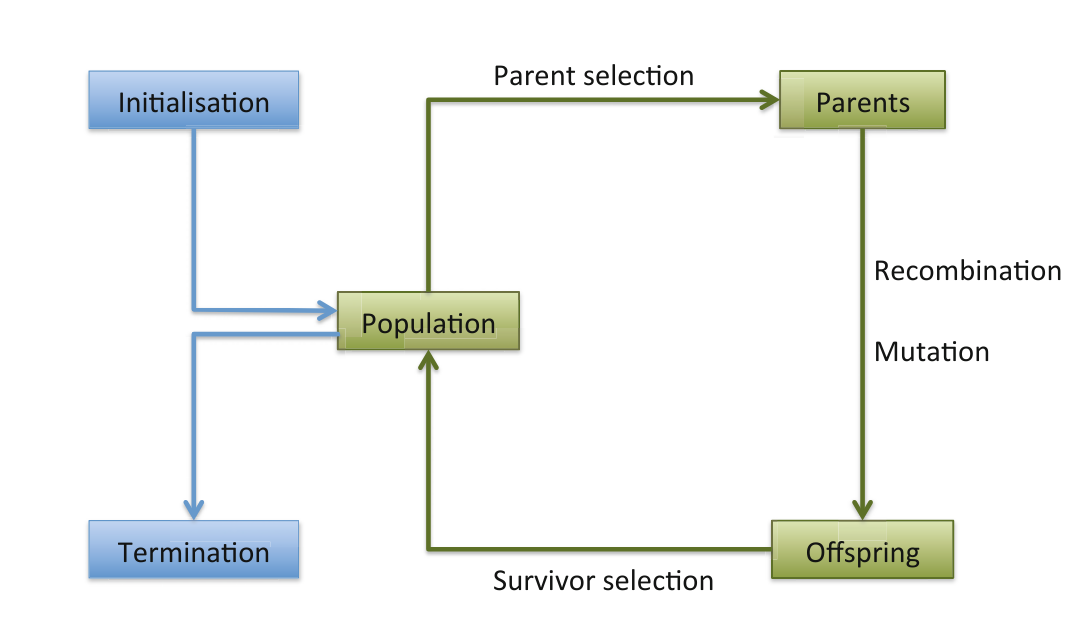
\includegraphics[width=1\textwidth]{EAFlowchart}
\caption{Evolutionary Algorithm Flowchart \cite{Eiben2015}  }
\label{ea}
\end{figure}
This algorithm is the most frequently used for deck building problems \cite{Fludal2017}\cite{GarciaSanchez2016}\cite{GarciaSanchez2018}, although they are optimized in different ways. In GAs, there exists a fitness function that determines the fitness score of an individual that is used to create the next generation, and there is the mutation function which will randomly mutate some individuals (it may or may not improve the fitness of said individual). \\ 
\indent Bjørke and Fludal \cite{Fludal2017} used a genetic algorithm to construct decks for Magic: The Gathering based on a certain pool of cards. Instead of using a fitness function that would calculate the score of a deck, they pitted each deck in that generation against each other in a tournament format using a Magic: The Gathering game simulator, each deck had the same number of games to play and they would select the fittest decks based of their win rate in the tournament. While theoretically, the idea is sound, the time that it took was substantial for an unremarkable win rate (less than 60\%). With 50 matches per deck over 350 generations, it took 43 hours to execute. Due to the time it takes, it would be unusable for players as it would simply take too long.\\
\indent Garcia-Sanchez et al. had a similar approach using lexicographical fitness with a Hearthstone game simulator called \textit{MetaStone}\footnote{\url{https://github.com/demilich1/metastone}}, separating the fitness evaluation into three parts: one part counted the number of victories of in 16 games, another part which determined the deck correctness (no more than 2 duplicates, only 1 legendary, etc...), and the last part was applying standard deviation to the number of victories, it being optimal if the deck won against every opponent \cite{GarciaSanchez2016}. The results were achieved faster much faster and were of a better standard than Bjørke and Fludal's work\cite{Fludal2017}, however, the results were not as high as they could have been, mainly due to the fitness function using \textit{MetaStone's} greedy AI to play. The decisions made by the AI would be greedy and different from that of a human player. The mutation function could also have been touched on, allowing the mutation to make smarter decisions about which cards to mutate. \\
\indent Garcia-Sanchez et al. tackled the problem once again and touched on the mutation function \cite{GarciaSanchez2018}, they developed a \textit{smart mutation} function that would replace a card in a deck with another of a similar cost (roughly ± 1). The results with the smart mutation were overall better than without it. This may solve one of the weaknesses of their previous work\cite{GarciaSanchez2016} but still uses the same greedy simulator heuristic.
\section{Machine Learning}
Machine Learning is a subset of Artificial Intelligence that constructs systems that can learn and improve without the need to be explicitly programmed. Burkov described it as "a subfield of computer science that is concerned with building algorithms which, to be useful, rely on a collection of examples of some phenomenon." \cite{burkov2019} \\
\indent This section of the review will present Machine Learning techniques that have been used or could possibly be used for deck building.
\subsection{Artificial Neural Network}
Artificial Neural Networks (ANN) also known as Neural Networks (NN) for short is an algorithm that was inspired by the biological neural networks seen in brains. They are a group of interconnected nodes or \textit{neurons} typically organised into multiple layers, an input layer, an output and \textit{n} amount of hidden layers. Through many loops known as \textit{epochs}, the NN trains itself using data from datasets to ultimately make a prediction based on given data as an input. Each node is weighted, and these weights are updated throughout the training process increasing the weight of positive output and decreasing on a negative one, allowing the system to make more accurate predictions \cite{3blue1brown}  \\
\begin{figure}[h]
\centering
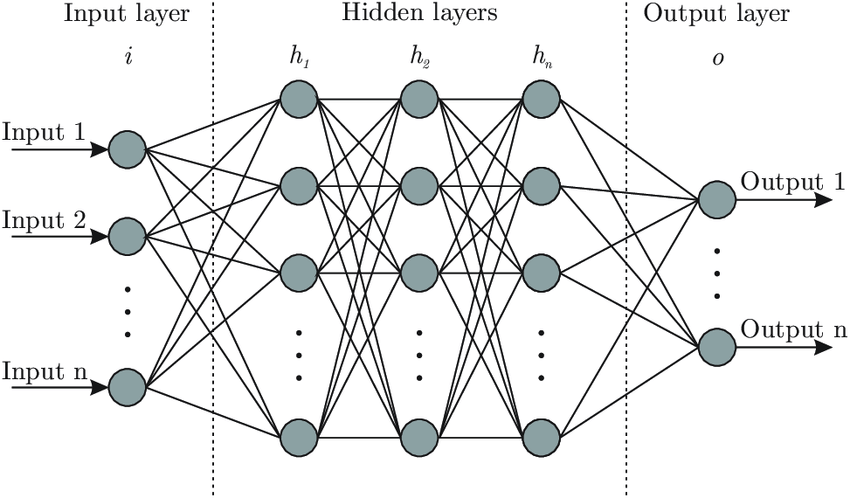
\includegraphics[width=1\textwidth]{ANN}
\caption{Artificial Neural Network architecture \cite{Facundo2017}  }
\label{ea}
\end{figure}
\\
\indent The approach to developing a deck-building AI is done differently than a GA. Ward et al. created a NN that emulated the choices a human would make when drafting a deck from a pool of cards for Magic: The Gathering \cite{Ward2020}. The idea was to select the cards that were chosen by a human in the dataset (target variable). The resulting accuracy on the test set was 65.7\%. The main drawback to this technique is that it requires the data to be clean, since the dataset used was a lot of decks drafted by human players, the data within may be suboptimal or purposefully tampered with, which would cause the AI to build weaker decks. \\
\indent Jakubik attempted a different method by using a NN to predict the win rate of a Hearthstone deck learned by using the results of observed matches \cite{NNWRPrediction}. This was a proposed solution to the AAIA’18 data mining challenge and came second. However, Jakubik's solution was subject to over-fitting, which Hieu Vu et al. tackled during the same challenge, which brought them the winning solution to the AAIA’18 data mining challenge\cite{PredictWR}. They tackled over-fitting by doubling the number of input features (or nodes) to account for the opposing player, they added an extra hidden layer and more test cases to compensate. Jakubik \cite{NNWRPrediction} and Hieu Vu \cite{PredictWR} rely on data of games that have already been played meaning that this method is not suitable for the construction of the decks rather the prediction of the win rate based on games that have been played. Ward et al. paper is the better technique of the three papers to build good decks, however, it requires clean and uncorrupted data.
 
\subsection{Generative Adversarial Networks}
Generative Adversarial Networks (GAN) is an application of generative modeling originally described in 2014 by Goodfellow\cite{NIPS2014}, which is an unsupervised learning task that automatically discovers patterns in the input data that the model can then use to output new examples that could have been drawn from the original data. A GAN uses a generative model to generate a similar output and a discriminator model uses supervised learning techniques to determine the probability of the generative output to be part of the training data\cite{NIPS2014}. The goal of the generative model or \textit{generator} is to create an output that can trick the discriminator into thinking it was part of the dataset. Goodfellow et al. use a fake money analogy: "We can think of the generator as being like a counterfeiter, trying to make fake money, and the discriminator as being like police, trying to allow legitimate money and catch counterfeit money"\cite{NIPS2016}. The GAN trains itself like this until the generator can create something that tricks the discriminator. Figure 1.6 shows the architecture of a GAN\\ 
\begin{figure}[h]
\centering
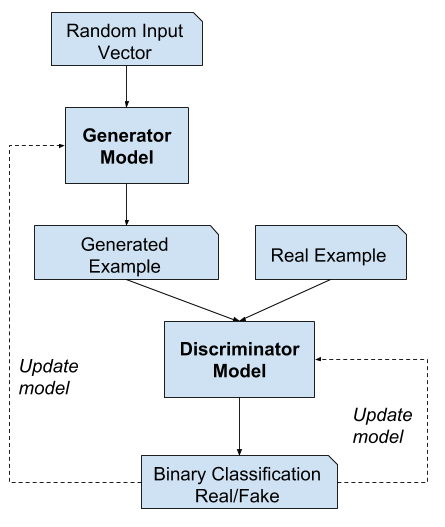
\includegraphics[width=0.5\textwidth]{GAN}
\caption{Generative Adversarial Network architecture\protect\footnotemark}
\end{figure}
\footnotetext{\url{https://machinelearningmastery.com/what-are-generative-adversarial-networks-gans/}}
\\
\indent As of writing this, there have not been any applications of a GAN for building decks. However, Rodriguez Torrado et al. combined a GAN with a procedural content generator to create different playable levels that were randomly generated from the generative model\cite{VGLG}. The GAN struggled to make playable and unique levels when provided a small amount of data. With this paper, it is theoretically possible to apply a GAN in a deck-building context but it will require a large amount of data to provide malleable results. 

\section{Hybrids}
In AI, aspects of a problem to be solved can be optimised through the use of multiple AI. This section of the review discusses papers that have used a combination of machine learning and evolutionary algorithms. The reason why GAs are combined with Machine Learning techniques is that GAs do not require lots of data to function, this allows for uses such as parameter optimization, Sehgal et al.\cite{Sehgal2019} uses GAs to speed up the learning process of their Deep Reinforcement Learning (RL) agent and provided the maximum success rate faster. Such et al. \cite{Such2017} used it for similar work, and stated that is was a competitive alternative to popular RL training techniques. It has also been observed that in the chemical field that the GA could outperform generative models in a discriminator neural network \cite{Nigam2019}, exploring the possibility of an application in GANs. The use of genetic algorithms in hybrid neural networks is mainly for achieving results faster \cite{Sehgal2019}\cite{Such2017}, however in highly parametrized systems the GA tends to struggle to find the optimal combination. \cite{Janikow1993}

%----------------------------------------------------------------------------------------
%	SECTION 3
%----------------------------------------------------------------------------------------
\section{Conclusion \& Final Thoughts}
This literature review has covered existing deck building solutions from Hearthstone and Magic: The Gathering, including evolutionary algorithms, neural networks, and various assistance systems. Potential solutions such as hybrid algorithms and Generative Adversarial Algorithms have also been discussed. Based on this literature review, it has been determined that evolutionary algorithms are the most popular method of tackling the problem therefore the most saturated of new solutions to explore. Machine Learning is a more obscure usage, focusing mainly on win rate prediction and card ranking. Hybrid algorithms and GANs have not yet been used in a deck-building context. In the context of GAs and NNs, they attempt to solve the deck building problem from different perspectives, the GA attempt to build a deck directly and test it in a simulated environment to determine the power of the deck in real-time, whereas the NN focuses on previous data that it uses to predict the power of the deck. They achieve the same goal, however, GAs are more direct and provided concrete results whereas the NN focuses on an indirect prediction from previous use cases. Moving forward this paper will explore solutions within those methods.


\chapter{Methodology}
\section{Overview}
The project implemented will be written in Python, in the form of three python notebooks, each with a specific task. The first notebook collects card data from an API and creates a card dataset, the second notebook scrapes deck data to create datasets for each class, and finally the last notebook will house the AI and the simulator testing. A user simply needs to run the notebooks to get their results, an input is required when deciding what class the user wants the deck to be. With the second notebook, additional datasets can be created and used in the place of the old ones for training the AI. \\ \\
This project outputs JSON files for the card and deck data, one file for the card data and ten files for the deck data (one for each class). When executing the AI, the user is presented with a certain number of decks, the number varies on how well the GAN trained, these decks are tested and the user is shown graphs and charts of deck composition, overall winrate and winrate per class. They can see the cards within the deck to use at their own leisure.
	
	%\renewcommand{\labelenumi}{\Roman{enumi}}
\section{Functional Requirements}
\begin{enumerate}
\item{ AI \textbf{MUST} output a legal deck following the rules of Hearthstone. Meaning that a deck should be composed of 30 cards, with no more than 2 duplicates of any card (excluding legendaries, which can only have a single copy).}
\item AI \textbf{MUST} output a deck following the rules of the "Standard" game mode. Meaning that the AI can only use the classic card set and the latest expansions from the past 2 years.
\item AI \textbf{MUST} use a generative adversarial network in order to generate a deck. The network will include a generator to create a similar and a discriminator to determine if the deck is part of the dataset.
\item AI \textbf{MUST} use a dataset of user created decks from the latest expansions in standard format (Rise of Shadows, Saviors of Uldum, Descent of Dragons, Ashes of Outland, Scholomance Academy, Madness at the Darkmoon Faire) collected from Hearthpwn.
\item AI created decks \textbf{MUST} be tested in a simulator to output a predicted win-rate and determine the playability of the deck versus user created decks. A total of 16 games should be played for optimal results. This will allow for the completion of requirement "f". 
\item The generated deck \textbf{SHOULD} have a calculated win-rate of over 50\%. Ideally around 60\%, so that the AI can make worthwhile decks. Meaning that the created decks should win at least half of the time, and in an ideal scenario they would win more often than lose.
\item AI \textbf{SHOULD} output a dataset of decks it generated following the same format as the training data, as to log the output and determine a possible bias.
\item AI \textbf{SHOULD} be able to generate a deck from a limited collection of cards, so it can be useful to players without access to all cards in Hearthstone.
\item AI \textbf{COULD} be used in the wild format, making use of all expansions to create competitive decks from a larger pool of cards.
		
\item An interface \textbf{COULD} be created to accommodate the AI and assist in feature implementation and accessibility of users. 
\end{enumerate}
\section{Non-Functional}
\begin{enumerate}
\item \textbf{MUST} have written consent from Hearthpwn to scrape data for dataset
\item Data collected \textbf{MUST} conform to GDPR regulations and be anonymous, since the identities of decks created by users is not needed.
\item \textbf{MUST} use Python as the programming languages of choice for the access to expansive libraries for data manipulation and AI creation.
\item \textbf{MUST} use Jupyter notebook as the software for coding the AI. It provides a platform for Python, and the cells are useful for making small changes without having to re-execute the whole program.
\item Dataset size \textbf{MUST} not be more than 100,000 rows as to decrease time to train and prevent overfitting.
\item The training process of the AI \textbf{SHOULD} take less than 3 hours, to allow a faster uptime if the AI needs to retrain after an update.
\item AI \textbf{SHOULD} use card data from the The Hearthstone API on RapidAPI if needed, to collected data such as card effects, images and tribal tags based of the name of the cards.
\item AI \textbf{SHOULD} use deck data scraped from Hearthpwn to train from using a coded web scraper.
\item Creation of a deck after training \textbf{SHOULD} not take more than 10 minutes. As to allow the to be quick to use by others whilst allowing for testing time with the simulator and the generation of graphs
\item \textbf{COULD} generate graphs of performance of decks outputted by the AI and simulators to visualise the training and testing process including the results of the created decks. 
\end{enumerate}
\section{Approach}
The project was designed using a agile methodology, equipped with logging, initially from a Trello board for the literature review and then migrated to github commit logs for the implementation of the project. The aim was to implement a requirement, testing it, fixing bugs and integration issues and adding additional features, this process was then repeated for each requirement until completion. \\ \\
Testing was done on a per feature basis, once a feature was implemented, a series of tests examples were created to ensure the functionality of it, if any errors or problems arose the focus would be shifted to fixing that issue. Evaluation was done after testing, once deemed ready, the AI was executed 10 times to create decks for each class which were evaluated over 100 games across all 10 classes, graphs then display these results.
\section{Libraries}
This section describes what libraries have been used in this project, the aim is to show transparency and understand some more ambiguous parts of the implementation. Note that all of these libraries are Python libraries.
\subsection{Web Scaper and API}
\subsubsection{Requests}
The requests library is a simple HTTP library that allows the user to send HTTP requests, whether it be GET or POST. This library was selected above others because over 500,000 others use this library aswell meaning that the library is stable and enables long term projects to stay active. This is used for both web scraping and api calls as both require to get a uri to get the information needed for the datasets.
\subsubsection{Json}
The json library allows for the encoding and decoding of json data, this is used for creating the outputs of the API calls and Web scraping, it is also used as an input for loading these data files and processing the data.
\subsubsection{Beautiful Soup}
Beautiful Soup is a library for web scraping, it pulls out data from HTML and XML files. There are three main libraries for web scraping, Selenium,  Scrapy and Beautiful Soup. Selenium is mainly used for AJAX requests and Web Application testing, so it is not ideal for this project as the request library is being used to make http calls. Scrapy whilst having more features, and being faster than Beautiful Soup, it is meant for complex web systems with middleware which are not needed in the scope of my project. Beautiful Soup was chosen for its simplicity and flexibility on small scale projects, since this will mainly be used for scraping data to create datasets. Originally Beautiful Soup was used for the collection of card data, it is no longer used for that as the resulting output was missing crucial data such as class, cost and image links, so an API for collecting the card data was used instead, which allowed the data to be stored in JSON format. 
\subsection{GAN}
\subsubsection{Keras}
Keras is a deep learning API that runs using Tensorflow, a machine learning platform which focuses on enabling speedy experimenting, it is simple to use and very well documented making it easy to implement models. This is what was used for the creation of the Generative Adversarial Network, specifically the implementation of the generator and the discriminator. 
\subsubsection{Numpy} 
Numpy is a python library designed for working with arrays, it aims to provide array objects that are 50x faster than standard python lists, since the GAN will be using a lot of arrays this is ideal for achieving faster training times. This library was used throughout the training process of the GAN, from sample generation to final deck results.
\subsection{Evaluation}
\subsubsection{Matplotlib}
Matplotlib is a data visualization library which allows data to be displayed through graphs and charts, this is used throughout the evaluation process of the project. 
\subsubsection{Time}
Time is a python library that is used to measure execution time of functions, in this project it is used to calculate execution time of the GAN training and testing process. 
\subsubsection{Fireplace}
Fireplace is the python library for the Hearthstone simulator, this is used for testing the generated decks against ones from the dataset. There are two other simulators worth considering, Sabberstone and Hearthbreaker. Hearthbreaker was used by the Google Deep Mind team for card generation however the project is no longer maintained, it has been for many years so that one cannot be used to fulfil our requirements. Sabberstone is written has a full interface but for testing that creates unnecessary bloat, so Fireplace is the better choice, it is maintained, and plays games in seconds, the main downside however is that only about half of the cards in the game are implemented. This is because some cards have tricky mechanics that are hard to implement and that the developers are to write interactions manually.
	
\chapter{Legal and Ethical Considerations}
Since data is a fundamental aspect to the success of the project, it is subject to certain legal and ethical implications that need to be addressed whether it be with the handling of the data or the collection of the data.
\section{Legal}
There are two main legal consideration for this project, the protection of data through GDPR and obtaining data through web scraping.
\subsection{Data Protection}
When dealing with personal data, developers are bound by laws to keep that data safe, the first most obvious law that needs to abided by is GDPR, which applies to the project since we are using EU data (among other countries aswell), certain protections must guaranteed. Some ways of protecting personal data are, pseudonymisation and anonymisation, in essence the user’s identity is protected by a pseudonym or with nothing at all which means that there will be no trace back to them, this could be represented as an ID or a username. If the data can be reversed back to personal data then data protection obligations will still apply, however if it is not possible then that data is no longer personal \cite{Euro2018}. Data minimisation should also be practised when dealing with personal data, this means that data should be lawful, fair, transparent and it should only involve data that is necessary for the task at hand, no more. So in the case only the essential information has been collected (deck data) to train the AI, it is completely anonymous. Data minimisation also extends to how the data is used, it should only be used for its intended purpose only and not to be shared to others. One final important legal implication I need to consider is usage of childrens data, since anyone can use my website I also need to consider the possibility of minors using the web system. GDPR covers specific safeguards for children, which include parental/guardian consent to children under the age of 16.

\subsection{Data Scraping}

The laws surrounding data scraping is a grey area, whilst not technically illegal, there can be issues around collecting personal data from open tabs or sites that require a log in. To stay on the right side of the law, best practise is to check their Terms of Service or equivalent, worst case of a breach could be a court case so it is in the best interests of every party to verify before scraping. The site that needed to be scraped for this project was Hearthpwn\footnote{\url{https://www.hearthpwn.com/}}, the data that needed to be scraped was public and pseudonymisation, since it was not behind a login page or any hidden pages it was not considered illegal. Before even writing the script, checking the Terms of Service of their site it said that data scraping was prohibited (Appendix A), this means that despite the data being public they do not want anyone using their data freely without permission. To get around this I sent an email to a representative of the site requesting permission to collect data for research purposes, after detailing the concept of the project and describing how the data would be used, the team at Hearthpwn granted me permission to scrape their site for data (Appendix B). 
	
	
	
\section{Ethical} 
This project raises certain ethical issues, raised from the collection of the user data, these issues are discussed below:
\begin{itemize}
\item Users may not know that their data is being used: Users may not be informed about their data being used to train the AI for this project.
\item Users may not realise the scale of which their data is being collected: Users may not know that a web scraping script was used to mass collect deck data to create a training dataset.
\item Users may not know how much information can be gained from analysing the data they have made available: Users may not realise that their data can be used to generate decks and data visualizations.
\item Users may not realise the rights a company has regarding their public data: Users may not be informed about the amount of control the company has on their data.
\end{itemize}
These ethical issues concern mostly the users of the Hearthpwn platform, other data used in this project is not user related therefore are not concerned by these problems. The terms and conditions of the Hearthpwn site state that any User Generated Content can be used, reproduced, modified, adapted, published, translated, transmitted, create derivative works from, distributed, performed and displayed by the Company or third parties in any way that they choose so long as the data is not deleted. \\

\begin{figure}[h]
\centering
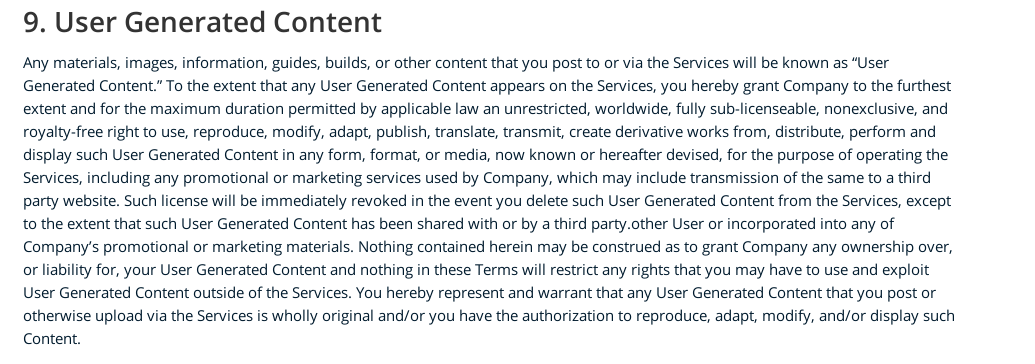
\includegraphics[width=1\textwidth]{ToS}
\caption{User Generated Content section of Hearthpwn Terms of Service\protect\footnotemark}
 \label{board}
\end{figure}
\footnotetext{\url{https://www.magicfind.us/terms/}}

The users of the platform need to be made aware of this, some of the issues listed above can be addressed but not all issues have a full solution. The ethical issues mentioned above depends on the user awareness to the extend of which their data is being used and the impact it may have, however, it would prove difficult to communicated to the whole user base of Hearthpwn that their data is being used. The best course of action would be to either used an official training dataset that is not considered personal data to allow for more public use or limit the extent of this AI to research and academic purposes, the latter being the best solution at this current time as an updated public dataset does not exist as of the creation of this project. 

\chapter{Implementation}
This section showcases the implementation steps of the project in three distinct sections: Card Data, Deck Data and Generative Adversarial Network. Each section will chronicle their respective development process, whilst discussing potential alternatives and limitations.
\section{Card Data}
\subsection{Introduction}
Before the development of the GAN can begin, data needs to be collected and formatted so that the GAN can be trained. The GAN can only take dimensional arrays as input, in the case of this project a vector, a single dimension array of numbers that identify specific cards to form a deck. From those deck vectors the GAN can learn, refine and generate new deck vectors that can be converted back into human readable form, resulting in a GAN created deck. In order to correctly identify the cards inside the deck vectors, going in and coming out of the GAN, a list of cards need to be compiled, each assigned with a unique numerical id that represents them.  
\subsection{Initial Method}
\subsubsection{Text File}
The initial method was to start of by creating a text file, this text file would contain a list of each cards that exists in the standard game mode of Hearthstone, each card would be separated by a line break within the text file. The aim is to make the file readable by a Python method, so that a dictionary can be created to identify the card by a integer key. \\
\\
\indent On the official Hearthstone website they have an online collection of every card in the game, these cards can be filtered and sorted by class, game mode, cost etc... This is a good source of information to gather the card data as it is official, reliable and up-to-date, this seemed useful as a list of card names could be compiled from scraping the site which could then be used to vectorize the cards for the GAN. The requirement for this project is that the GAN must create standard decks from the past 2 years, so filtering to standard is necessary. \\

\begin{figure}[h]
\centering
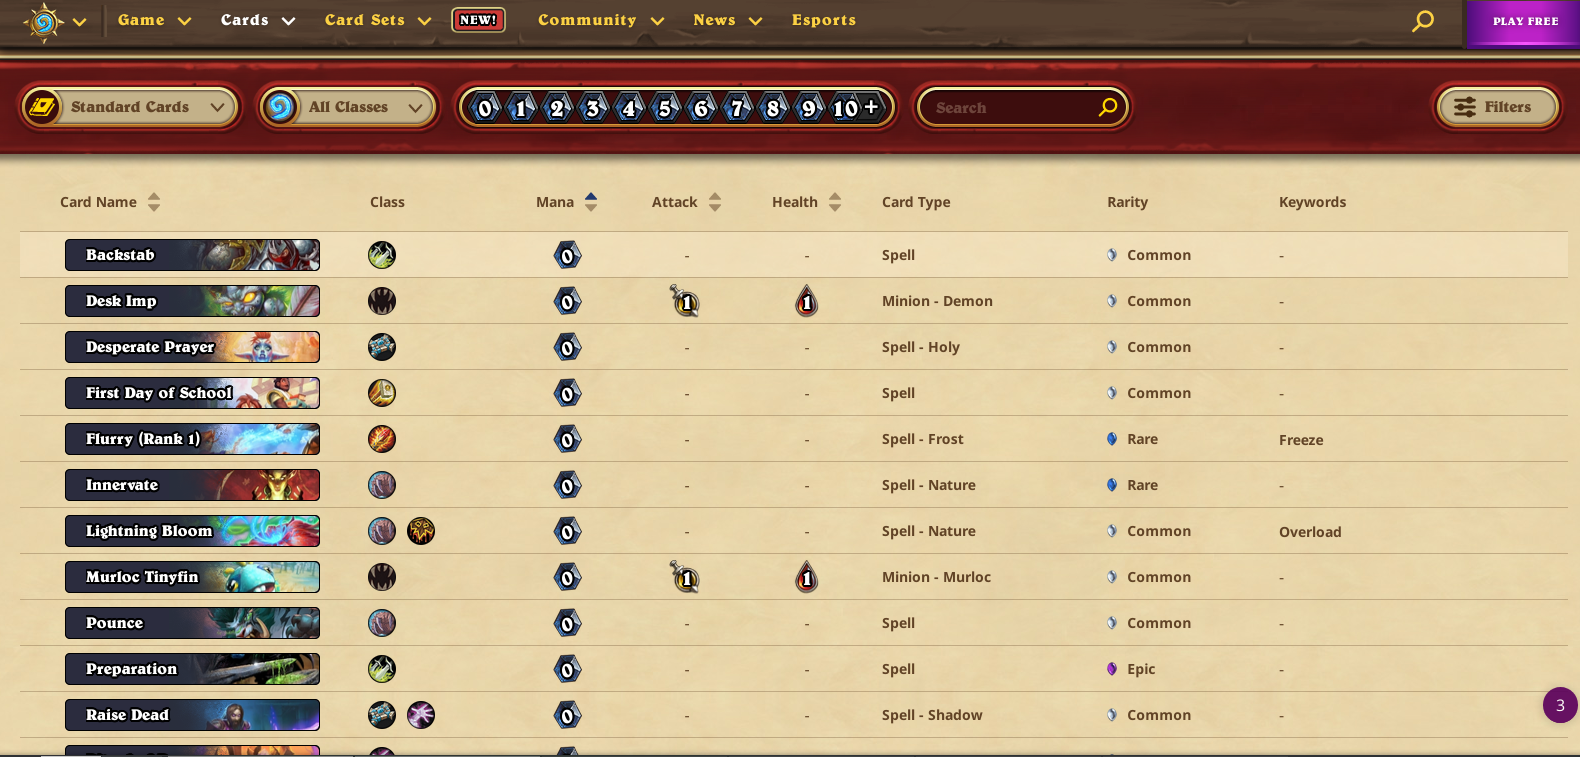
\includegraphics[width=1\textwidth]{collectionpage}
\caption{Hearthstone Collection Page\protect\footnotemark}
 \label{board}
\end{figure}
\footnotetext{\url{https://playhearthstone.com/en-us/cards}}


\indent Collecting the card data using the Beautiful Soup library proven futile, the site has a maximum card display setting meaning that only a small portion of the cards are displayed at one time, the rest are loaded by continuously scrolling to the bottom of the page. Due to the simple nature of the web scraper, it could not load the rest of the cards by scrolling (if the page was using different pages instead then it would have been possible to collect them), resulting in it only collecting a tiny portion of the standard cards. A solution was found by using a firefox web extension called "Open Web Scraper"\footnotemark. \\ \\
Open Web Scraper is a scraper add-on that appends onto the web developer tools of a web browser. The user can then create a sitemap by entering a URL, then from this sitemap, the user can query information from the entered URL. After looking at the source code of the Hearthstone page, a query was written to get the name of every card on the page that was loaded beforehand with all the standard cards loaded. The query was \nolinkurl{tr:nth-of-type(n) div.CardTableLayout__CardCropCell-sc-1jy3g9y-}, in short the query gets all names from the CardTableLayout table. The results are then highlighted in red on the page. These highlighted areas were then saved to a text file called cards-standard.txt (which can be view in Appendix C).

\begin{figure}[H]
\centering
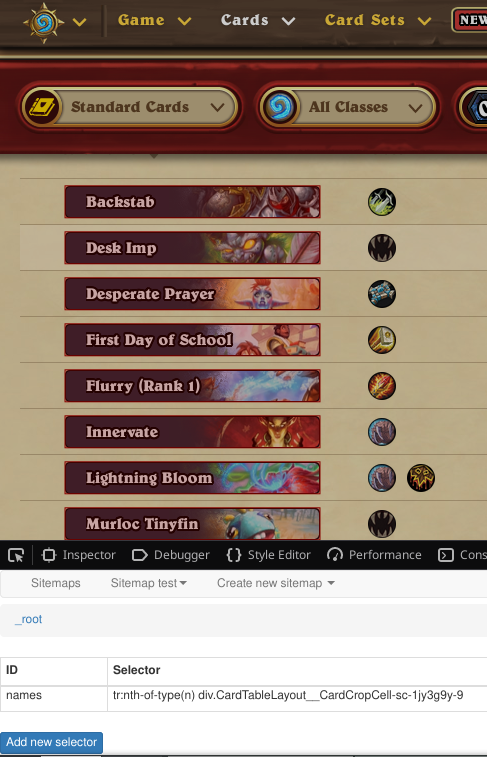
\includegraphics[width=10cm,height=10cm,keepaspectratio]{OpenWebScraper}
\caption{Open Web Scraper Results\protect}
 \label{board}
\end{figure}
\footnotetext{\url{https://webscraper.io/}}

\subsubsection{Implementation of Initial Method}
Once the \nolinkurl{cards-standard.txt} file was created, the implementation of the card vectorization could begin. Using Python the file was opened and with the \nolinkurl{readlines()} method, an array of each card name was created. Two dictionaries were then created for the purpose of converting the cards to id form and back, the first dictionary called \nolinkurl{cards_key} housed the names of the cards which could be searched by id and the second dictionary called \nolinkurl{cards_value} did the inverse, allowing the id to be found by searching the name.

\begin{figure}[H]
\centering
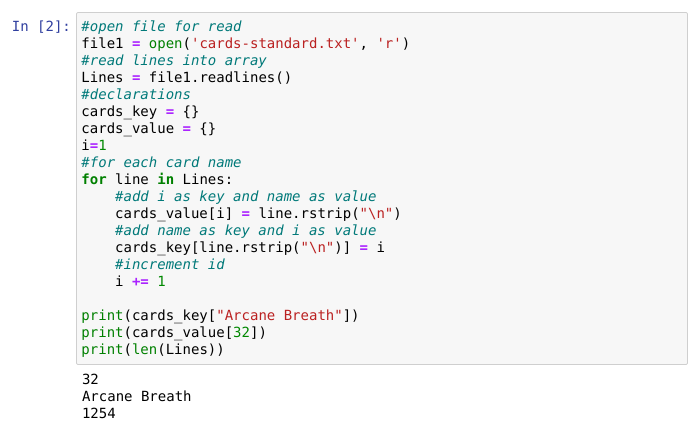
\includegraphics[width=1\textwidth]{InitialFileRead}
\caption{Code Extract of dictionary initialization\protect}
 \label{board}
\end{figure}

With the two dictionaries created, the functions that allow created decks to be vectorized or converted to readable form need to be integrated. Two functions, one to vectorize called \nolinkurl{deck_to_vector_csv} , another to de-vectorize called \nolinkurl{vector_to_deck_csv}. Both use a loop but they use different dictionaries to get the card in the desired form then an array of the converted deck is returned. Although there is some text pre-processing done beforehand when vectorizing the decks, unwanted white spaces can causes bugs in the future so by using \nolinkurl{lstrip} and \nolinkurl{rstrip}, excess white spaces on the left and the right of the card name can be removed (this does not include spaces between words).

\begin{figure}[H]
\centering
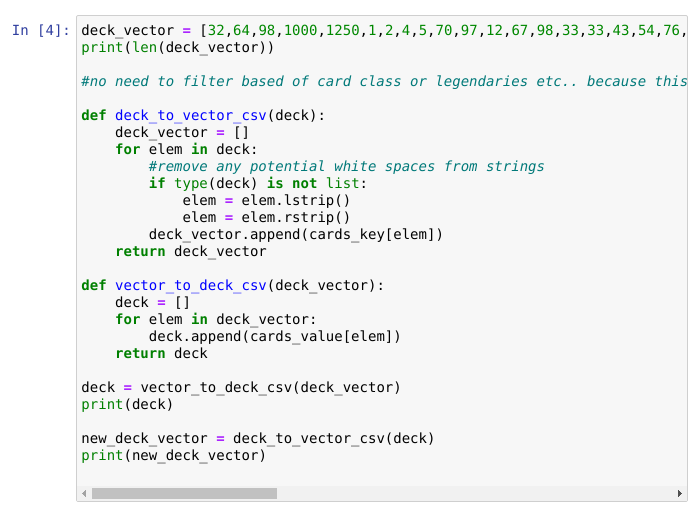
\includegraphics[width=1\textwidth]{deckConversion}
\caption{Code Extract of deck conversion functions\protect}
 \label{board}
\end{figure}

The result is a functioning card and deck vectorization and de-vectorization system that will allow the deck data to be converted into a format that the GAN can train with, and return the generated decks to human readable deck without loss of information throughout the process.
\subsubsection{Limitations}

Whilst this method functions without issue, there are certain limitations it. The main limitation is that the only information displayed about the cards is their id and their name. This is not enough information to do evaluations, sorting, displaying or even class selecting, meaning that with this method there would be no way of determining the validity of the deck, check for mana curves, check type split. Another limitation is that there are some libraries like the simulator that use official Hearthstone card id's to identify cards and use them to play simulated games. So a new method would need to be adapted to incorperate these changes. This would also allow for easier, more flexible expansions on the project in future works.
\subsection{Improved Method}
The new method will make use of third party platforms that already have the data needed to train the AI. The format of this file will be JSON, it is the easiest format to parse, there are many libraries in Python that enable the processing of JSON data. There are many ways of obtaining this data, this next section will describe three potential platforms to get the card data from, and then select one based on their pros and cons. Once the data is collected into a file, then it is simply a matter of loading the file, all the data will be correctly structured and available. Some data cleaning will likely be needed. 
\subsubsection{Blizzard API}
The Blizzard API is a platform that allows a user to gather information about any of their games, the one that interests the project is the Hearthstone section. On this the user can make card searches, gather metadata and even use their deck code algorithm that turns a deck of cards into a string that can be copied and used to instantly build a deck in the game. \\
\indent The upside to this API is that it is official, so it will likely be maintained and updated frequently far into the future, however, the downside is that the API is designed for web application so it requires OAuth with a secret client to generate a token to use the API. This would disallow anyone other than the client user to make use of the implemented code, since the client ID is limited to a single person, and for security reasons that client ID cannot be given, this process makes it awkward for other developers to make use of the code. \\ 
\indent Another downside is that the API is extremely limited in the data that can be collected from it, the data needed for the project is a list of cards, but the Blizzard API only allows a single card search at a time meaning that a list of card names would need to be compiled then an API call will need to be repeated for every card (which at the moment with current standard cards is 1254 times). Although thanks to the initial method a list of card names has already been compiled, so it would be feasible to gather the data from this API is a way around the OAuth can be found. The API throttles at requests at a rate of 36,000 requests an hour, albeit many request if exceeded it would block the API from being used further until the next hour, this can be problematic if the secret client ID were to be shared along with the code to a public platform, if too many users were to make requests at once it could block users out of the API.

\subsubsection{HearthstoneJSON}
HearthstoneJSON is a web site that considers itself an API, it functions differently to an API because on the site there are a series of file uploads each one after an update (like an expansion release) with the new cards, there are two files that are uploaded each time, one with all the cards and other with just the collectible cards. The cards that interest us are the collectible ones as the other non-collectible cards are tokens or cards that other cards generate and cannot be added manually to a deck. This API does not allow the user to make queries for specific card data, it is simply a file with everything in it, this is both a good and a bad thing, it makes the data collection easy since all that is needed is to download the file but it means that cards will have to be manually sorted, wild from standard, specific sets, etc... \\
\indent Furthermore, it means that no code is required to gather the data, however, a user would need to download the file if they want the new cards and it heavily relies on the developers staying up to date with it. As of now, the api has not been updated since 2018 signifying that that it does not have the latest cards making it tricky to fulfill the standard cards only requirement.

\subsubsection{Hearthstone API}
Hearthstone API is another web platform that makes use of RapidAPI for their endpoints. RapidAPI is a site that hosts thousands of API's that can be accessed with a single key, it allows users to make queries either on their site or through a library to gather data. Hearthstone API relies on this platform to allow users to make queries, unlike the Blizzard API, there search options are limitless, a user can search for specific expansions, collectible, card name, card class and much more. The API is constantly updated, so that even the latest released cards are added, there still is the issue with the access token, but it is more manageable  since a developer can use their RapidAPI key from their account, or an account can be created, no OAuth needed. The biggest downside is that the API has quite high latency, meaning that it would take longer to make API calls.
\subsubsection{Choice}
All three platforms have their pros and cons for their usage, however the better one to choose would be the Hearthstone API using RapidAPI. The reasons are because, it is updated and actively maintained unlike HearthstoneJSON, it also allows to do queries to limit the range of data gathering to what is needed so in theory no pre-processing will need to be done. Access to Hearthstone API is also easier to its Blizzard counterpart because of the RapidAPI platform and the lack of OAuth which is not needed in the context of this project. The JSON data that the Hearthstone API provides will encourage sorting and filtering to improve the GAN training. To summarise, for this project the best choice is Hearthstone API due to how updated it is and how much easier it is to use compared to its respective counterparts. 
\subsubsection{Implementation of Improved Method}
To get the data from Hearthstone API, the \nolinkurl{requests} library was used to access the RapidAPI platform. The data was collected using the Card Sets query built into the API which allows the user to get all the cards from an expansion. An array of these expansions was created and iterated through to make a query for each card set, the result was an array of card lists per expansion. Once that was created, the card lists were concatenated into a single array whilst adding an integer id that will be used for the GAN model. Finally, the JSON list was written into a json file using the \nolinkurl{json.dump()} method from the \nolinkurl{json} library.

\begin{figure}[h]
\centering
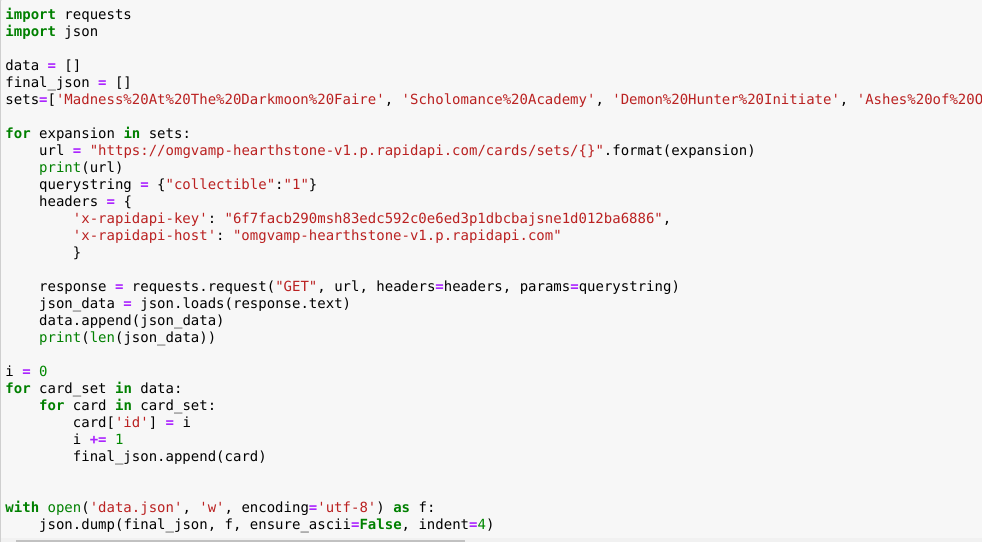
\includegraphics[width=1.25\textwidth]{cardAPI}
\caption{Getting card data with Hearthstone API\protect}
 \label{board}
\end{figure}

The file created is a json file called \nolinkurl{data.json}, an extract of the contents can be viewed in Appendix -- .  Loading this file for the GAN is straightforward, simply use the in-built Python \nolinkurl{open()} function. As seen in figure 5.6 below the amount of information provided by a single card is a big improvement to just the name of the card.

\begin{figure}[H]
\centering
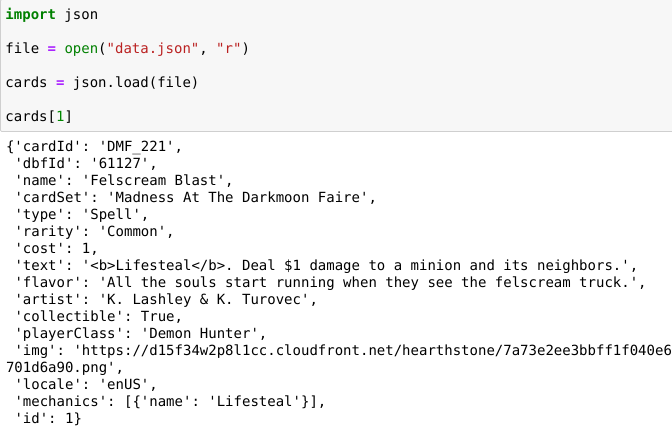
\includegraphics[width=1\textwidth]{jsonOpen}
\caption{Loading card data\protect}
 \label{board}
\end{figure}

Whilst working with the collected data, some minor inconsistencies appeared in the JSON, firstly the name of hero portraits appeared, these are special personas a class can take on, with different animations, audio queues, however they are not cards, those outliers need to be removed for the code to function. Another issue stemmed from the latest expansion \textbf{Madness at the Darkmoon Faire}, this expansion added a new type of card, the dual class card, allowing two different classes to use the card, the problem is that due to the structure of the JSON there can only be a single class under the key \nolinkurl{playerClass} (which can be seen in figure 5.6). To fix these issues, a function was written to remove the hero portrait outlier cards, and append both classes of dual class cards to a variable. 

\begin{figure}[H]
\centering
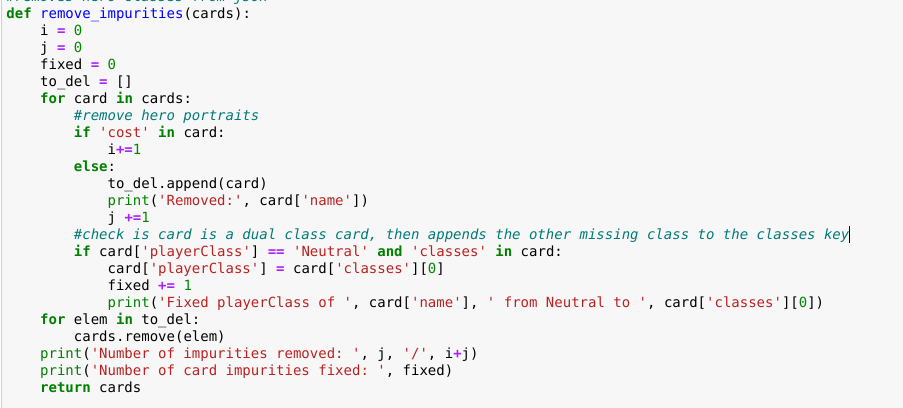
\includegraphics[width=1.25\textwidth]{impure}
\caption{Removing impurities in card data\protect}
 \label{board}
\end{figure}

\section{Deck Data}
\subsection{Introduction}
The core necessity for the success of the project is data, the GAN requires a lot of data to train, a lot of deck data. Datasets do exist and can be found on various platforms, however they tend to be outdated or limited in size. The GAN takes the datasets as input for the discriminator to use to determine if the generated decks are similar. So where can recent datasets for Hearthstone decks be found? Well unfortunately ready made datasets for the specific purpose of this project, however, platforms exist in the hearthstone community where the users post their decks online, these decks can be rated, sorted and viewed. Using a web scraper would enable the gathering of the deck data needed for the GAN. Web scraping is a technique for harvesting data on a website, the tool used to accomplish the task is called a web scraper among other names. Legal issues surrounding web scraping can be found in Section 4.1.2 of the report.
\subsection{Platform Choice}
HSReplay and Hearthpwn are the two most popular sites in the community, Hearthstone players frequent these sites to see what decks are strong currently or to find niche archetypes to accommodate the use of certain cards they like. This sub section will describe both platforms and which one is the better fit in the context of this project.
\subsubsection{HSReplay}
HSReplay is a community run website owned by HearthSim (the same people that have developed the Hearthstone simulators), the most notable feature is their game replay feature, allowing users to view and share their previously played games. They also provide extensive statistics about cards and decks based on user played games. \\ \\
The site has a lot of features, graphs and statistics, but all of this is not really useful as the dataset only needs the decks themselves. The biggest downside to this website is how they display their data. After sending a request to scrape data from their site, getting data from their site proved tricky, due to all the features and displays, the data does not seem to be loaded straight away, meaning that the web scraper can not seem to find certain information, namely the deck lists. The deck lists are requested after the page has loaded to prevent the web page from taking to long to load, whilst this is good practice to improve the sites usability, it impedes the web scraper.  Before delving any deeper into the issue, testing the second platform might prove to be more straightforward. 

\subsubsection{Hearthpwn}
Hearthpwn is an alternative to HSReplay, it acts as a database for cards and decks rather than statistics and replays. Decks can be sorted by expansion, popularity and class. This site's features can actually assist a web scraper in collecting the data that is needed. Because of the sites minimal design it runs smoothly and loads fast, so from first glance it seems ideal for data harvesting. After receiving permission to collect data, initial testing was successful and much less hassle than HSReplay, because of this the best course of action is to select Hearthpwn, for the in depth sorting and simplicity to scrape. The next sections will detail methods to scraping data from Hearthpwn.
\subsection{Initial Method}
Before speaking about the implementation of the web scraper, the first thing that needs to be discussed is the way it was formatted initially and how it was improved. Since the web scraper implementation is the exact same for both the initial and the later improved method, the web scraper code can be explored further on.
\subsubsection{Text}
The initial method made use of the \nolinkurl{cards-standard.txt} file that was reviewed before, this is because the web scraper was initially implemented with the text file method in mind then was later changed to accommodate the improved system. The idea is that the web scraper collects the deck data and then stores it into two separate arrays, the first one to store the deck list, so every deck with their card names inside them and the second one is the class of the deck. The reason why there are two arrays was to create a dataset for each class, in order to organize the training of the GAN. These arrays would then be sorted by class, then a \nolinkurl{csv} file containing the deck data would be saved. For safety, the datasets were saved in a vectorized and non-vectorized form, it was unknown which one would be better or easier to use so both forms were saved.
\subsubsection{Implementation}
\begin{figure}[H]
\centering
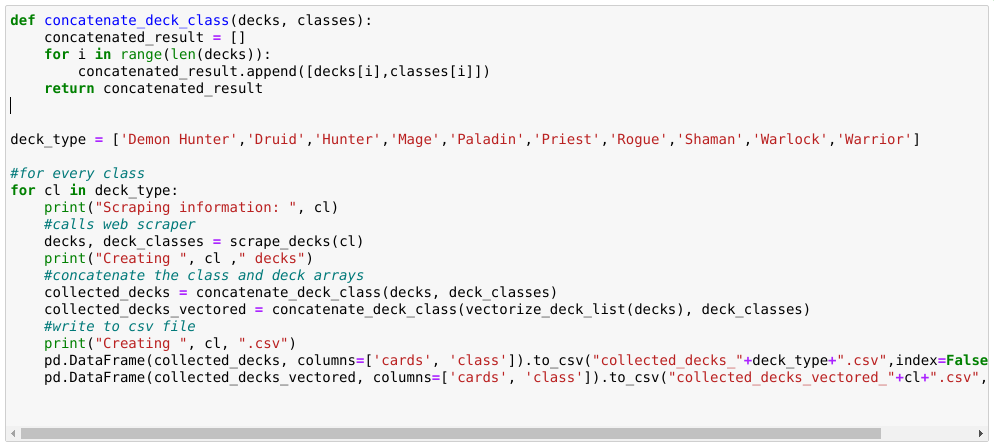
\includegraphics[width=1.25\textwidth]{csvIm}
\caption{Writing scraped data to csv file\protect}
 \label{board}
\end{figure}

The implementation follows after the collection of the data into the two arrays, a concatenate function was then created to append the class label to the deck list, the file writing was done using \nolinkurl{pandas} to create a dataframe to then save the file as a csv. An example output csv file can be seen in Appendix E \\ \\

With the csv files created and filled with data, the decks within need to have a way to be extracted, so that they can be used in the GAN. When reading the file, anomalies were checked for: problematic characters, excess brackets and deck length. Since the standard size of a legal deck is 30 cards, any that do need reach that will not be used for training, the result is an array with the deck lists and their class labels. However it was later on discovered that the class labels would not be enough to correctly build the GAN, since there can be other class cards or neutral cards in a deck list, hence why the JSON method was implemented later on. 


\begin{figure}[H]
\centering
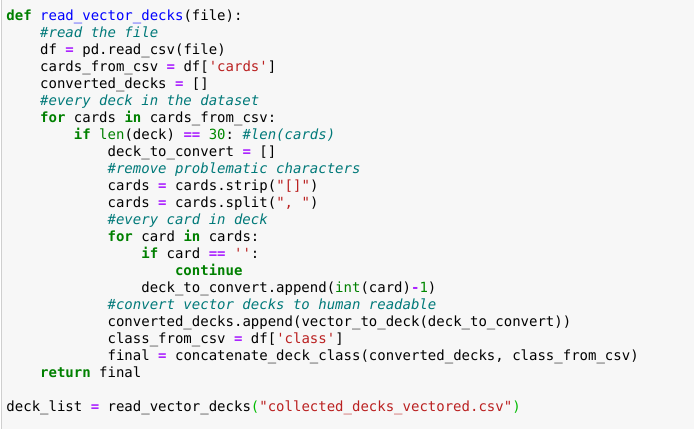
\includegraphics[width=1.25\textwidth]{readVectorDecks}
\caption{Reading csv file\protect}
 \label{board}
\end{figure}


\subsection{Improved Method}
In the previous section, the project was making use of already vectorized deck data from the web scraper. The problem with that is that if the card list is changed in any way, for example when sorting by a certain class, or removing impurities, the indexes of the vectors will be wrong. So it would be better to save them in a human readable format, then vectorize them when needed. However using \nolinkurl{csv} file format, data will be harder to read, even with just the integer numbers, a decent amount of pre-processing was required to just read the data. Using another method may save time and processing power, good thing is that there is a better alternative with the JSON card data that was collected previously. By loading the \nolinkurl{data.json} card data file, with just the names of the cards a JSON dataset can be created by converting the web scraped card names to full fledged JSON data format.
\subsubsection{Implementation of Improved Method}

To begin, the code for the \nolinkurl{csv} conversion needs to be adapted, it will be longer than with the csv. Instead of vectorizing the deck data and then writing to file, the scraped data is appended to a \nolinkurl{to_convert} array. An example of a scraped deck looks like:
\texttt{['Lab Partner', 'Lab Partner', 'Primordial Studies', 'Primordial Studies', 'Wand Thief', 'Wand Thief', 'Astromancer Solarian', 'Cram Session', 'Cram Session', 'Runed Orb', 'Runed Orb', 'Wildfire', 'Wildfire', 'Firebrand', 'Fireball', 'Fireball', 'Reckless Apprentice', 'Reckless Apprentice', 'Refreshing Spring Water', 'Refreshing Spring Water', 'Ring Toss', 'Ring Toss', 'Jandice Barov', 'Ras Frostwhisper', 'Flamestrike', 'Flamestrike', 'Mordresh Fire Eye', 'Far Watch Post', 'Far Watch Post', 'Taelan Fordring']}


The JSON card data is also loaded for the conversion later on.
\begin{figure}[H]
\centering
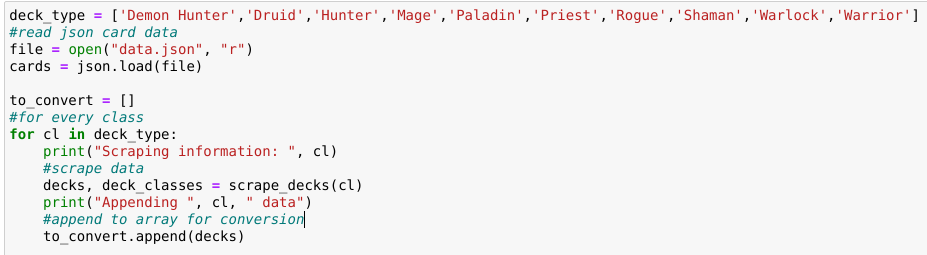
\includegraphics[width=1.25\textwidth]{improvedDC}
\caption{JSON adaptation of previous code\protect}
 \label{board}
\end{figure}

To convert the scraped data to a JSON format, the name of the cards need to be searched through the \texttt{cards} array, then a new list needs to be created to add the converted cards into. Figure 5.11 is a code extract of this process. For each card in a classes deck list, strip excess white spaces then find the name of the card in the JSON card list, once found append to a new array. Once the conversion is complete, the data is then written into a JSON file using \texttt{json.dump()}. Then the creation of the dataset is complete. An extract of the a converted JSON dataset be found in Appendix F.

\begin{figure}[H]
\centering
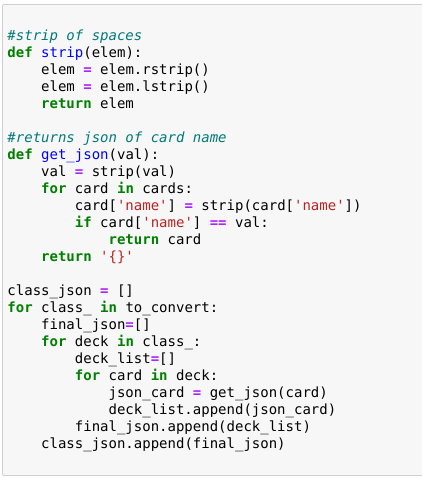
\includegraphics[width=9cm, height=10cm]{JSONConversion}
\caption{JSON adaptation of previous code\protect}
 \label{board}
\end{figure}

Since the file type for the datasets has changes from \texttt{csv} to JSON, it means that the file loading needs to be modified to work with the updated datasets. Luckily it is straightforward to load JSON data, with the \texttt{json} library, simply load the file (as seen in figure 5.12), there is also a check to only register decks of legal length.

\begin{figure}[H]
\centering
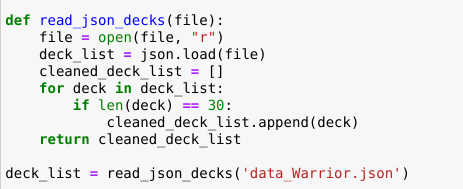
\includegraphics[width=1\textwidth]{readJSONDecks}
\caption{Read JSON file\protect}
 \label{board}
\end{figure}

\subsection{Implementation of Web Scraper}
Now that the methods surrounding the web scraper have been detailed, the implementation of the web scraper can begin. Firstly, the library that is used to get the data is \texttt{requests}, and the library that is used to parse through the data is \texttt{Beautiful Soup}. Before harvesting the data, the url needs to be determined for the request method to work, since there are 10 classes in Hearthstone, 10 separate urls will be needed. The urls are uncomplicated to find, figure 5.13 shows the filter section of the deck search on Hearthpwn. Every class has a unique id when attempting to filter: \texttt{'Demon Hunter' : 16384,
          'Druid' : 4,
          'Hunter' : 8,
          'Mage' : 16,
          'Paladin' : 32,
          'Priest' : 64, 
          'Rogue' : 128,
          'Shaman' : 256,
          'Warlock' : 512,
          'Warrior' : 1024}\\
So a dictionary was created to store these values so that when the web scraper goes to collect a certain class decks, it can find the values easily. An example url will look like: \nolinkurl{https://www.hearthpwn.com/decks?filter-show-standard=1&filter-show-constructed-only=y&filter-deck-tag=1&filter-class=4)}. This link will only show standard and constructed decks, \texttt{filter-deck-tag} sorts the decks buy \texttt{"hot"}, which means popular decks and of course the class filter, in this example it is Druid decks.
\begin{figure}[H]
\centering
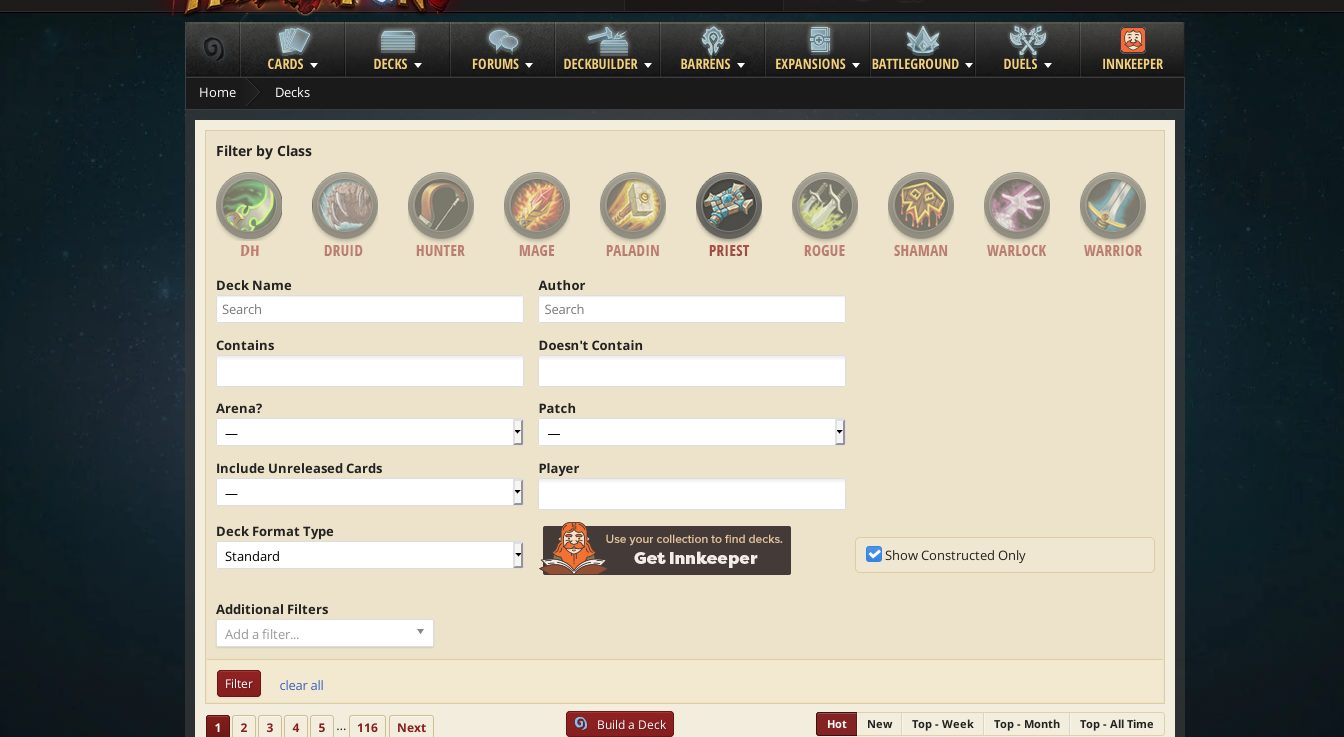
\includegraphics[width=1\textwidth]{HSpwnDecks}
\caption{Hearthpwn deck search\protect}
 \label{board}
\end{figure}

The links though will only display the first page of decks, which is around 25 decks per page, the are many more but the number is not fixed, so before the decks can be collected, the number of pages there are needs to be found, \nolinkurl{page_max} does just that (figure 5.14).

\begin{figure}[H]
\centering
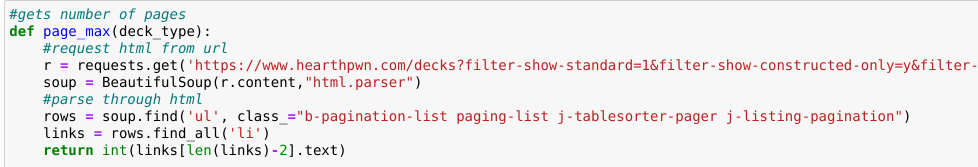
\includegraphics[width=1.25\textwidth]{pageMax}
\caption{Function that finds the number of deck pages there are\protect}
 \label{board}
\end{figure}

The scraping needs to be done in two parts, this is because the results shown on the deck search page does not include the cards that are use to build the deck, that is hidden behind another link to the deck information. This means that initially, the links to the decks needs to be collected, then another part needs to go within those collected links to harvest the card data. The \nolinkurl{scrape_decks} function takes a class as an argument and creates the starting links for the selected class and gets every deck link, from all the pages (figure 5.15). 

\begin{figure}[H]
\centering
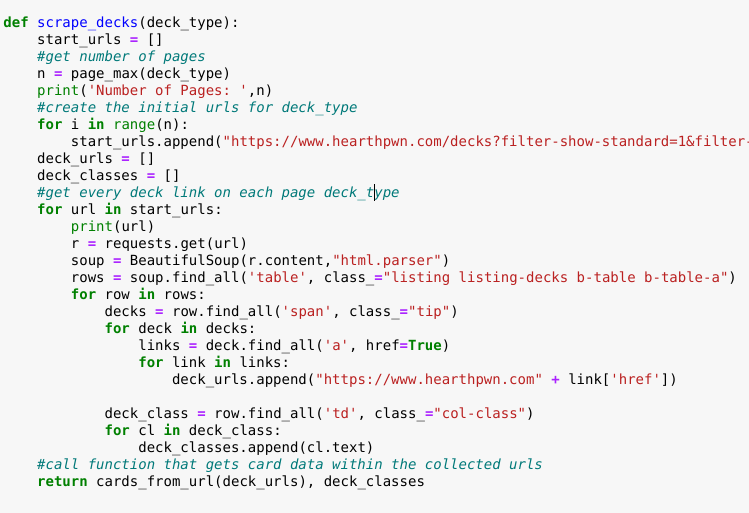
\includegraphics[width=1.25\textwidth]{scrapeDecks}
\caption{Gets all deck links from class page\protect}
 \label{board}
\end{figure}

After the deck links are collected, another function called \nolinkurl{cards_from_url} is called, this take the urls as an argument and returns the deck lists in their default format (figure 5.16). It navigates thorough the page into the html table containing the list of cards and gets the names. Finding the correct tables and containers was found through trial and error, but is consistent throughout every page on the site.

\begin{figure}[H]
\centering
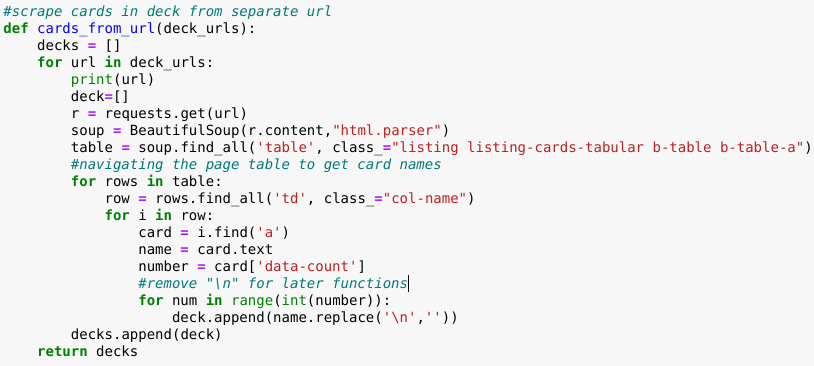
\includegraphics[width=1.25\textwidth]{cardsURL}
\caption{Gets cards from deck links\protect}
 \label{board}
\end{figure}

\section{Generative Adversarial Network}
\subsection{Introduction}
When researching GANs, the main application that they were used for was image generation with human and artistic applications, creating realistic people that do not exist from many images of people. The GAN made use of libraries to convert the images into two dimensional arrays, single dimensional arrays seemed scarce at best. Only a few basic tutorials about vectors in a two dimensional space could be observed using single dimensional input. Making use of what little information about single dimension GANs was available, the conversion from 2D to 1D started. The vectorization of decks idea was thought of when the conversion of images was observed. The point is that by feeding the GAN many vector inputs, the resulting output will be a vector that is similar to the training vectors but different enough for it to create unique vectors, whilst demonstrating "thinking" on the GANs part. (talk about tutorial that inspired me and reference it)
\subsection{Implementation}
The structure of the implementation is as follows, to begin the generator and discriminator models will be define, then how it combines into a GAN, after that the training process will be discussed, finally the performance summary will be detailed.
\subsubsection{Generator}
The generator is a sub-model of the GAN that will generate the deck vectors. The generator is composed of layers, an input layer, an output and activation layers between. A dropout layer is also added to the generator to help prevent over-fitting by randomly setting inputs to 0 during training time. The number of activation layers added to the generator is the result of many hours of optimization, when training graphs are displayed showing how similar the generated deck is to a real deck. After hours of tweaking, one input layer, one output layer and two activation layers (of 200 activations) seems to produce the best outcomes. All the layers except the output layer are \texttt{ReLU} activated, this limits the vectors from going into the negative numbers. The output layer is set to \texttt{linear} otherwise if there are any card ids generated that do go into the negative, they will automatically be set to 0 which is a card id itself. The generated negatives numbers and how they are dealt with is discussed later on. The loss is calculated through \texttt{binary cross-entropy}, because it categorizes a deck to be either 0 (a fake deck) or 1 (a real deck). Figure 5.17 shows the code implementation of what was described, the \nolinkurl{Sequential} function is part of the \texttt{keras} library function to declare the model, \nolinkurl{Dense} and \nolinkurl{Dropout} as also part of \texttt{keras}.

\begin{figure}[H]
\centering
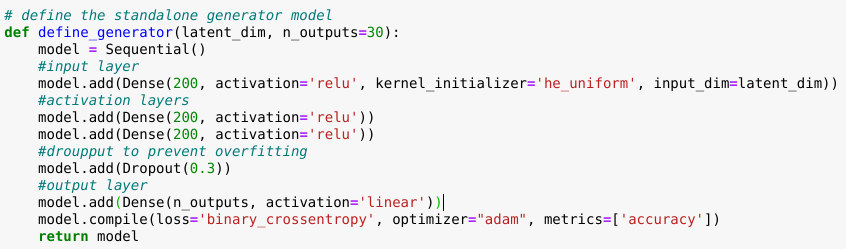
\includegraphics[width=1.25\textwidth]{generator}
\caption{Define generator model\protect}
 \label{board}
\end{figure}
\subsubsection{Discriminator}
The discriminator is the second sub-model that constitutes the GAN, the purpose of the discriminator is to determine if a deck vector created by the generator resembles the deck vectors from the training dataset. The model is smaller than a generator model with just an input and an output layer. The input layer has 30 activations and take a generated vector with 30 inputs (the amount of cards within deck) with \texttt{ReLU} activation. The output layer has a single output and a sigmoid activation, this is because the output of the discriminator is a binary result, 0 for fake, 1 for real. This sub-model is also reliant on \texttt{binary cross-entropy}. Figure 5.18 is a code snippet of the discriminator illustrating the explanation.

\begin{figure}[H]
\centering
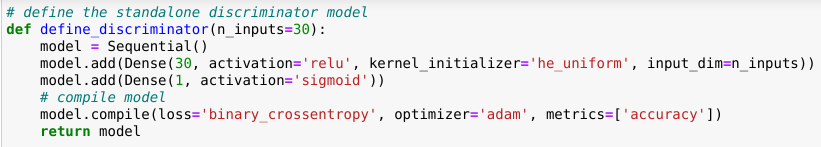
\includegraphics[width=1.25\textwidth]{discriminator}
\caption{Define discriminator model\protect}
 \label{board}
\end{figure}

\subsubsection{GAN}
The GAN section is where both the generator and the discriminator sub-models are added to the GAN model. There is also a setting that needs to be changed, the discriminator needs the weights to not be trainable or the criteria of the discriminator will change and disrupt the training process. 

\begin{figure}[H]
\centering
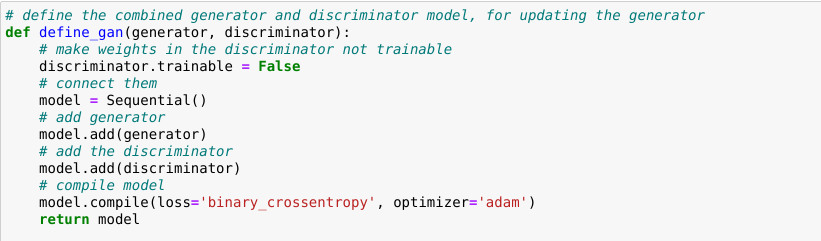
\includegraphics[width=1.25\textwidth]{gan}
\caption{GAN model\protect}
 \label{board}
\end{figure}

\subsubsection{Training}
This section is where the training of the GAN happens. The training process starts off by preparing the real and fake decks, the real ones are sampled from the dataset randomly and the fake decks are generated randomly (not by the generator). The results from these functions return an \texttt{x} and a \texttt{y} variable, so \nolinkurl{x_real}, \nolinkurl{x_fake}, \nolinkurl{y_real} and \nolinkurl{y_fake}. The \texttt{x} variable contains the array of deck vectors and the y their labels, their labels being a binary to help the GAN distinguish if they are a real or a fake deck. After the real and fake decks are gathered, they are used to update the discriminator model, so that it can distinguish real decks from fake decks. \\
Once the discriminator model has trained, the generator creates a deck vector to attempt to trick the discriminator. The deck is then trained on the GAN model to update the generator based on the discriminator's error.  \\
The whole process is repeated for the number of epochs given, for this GAN model it is 10,000 epochs. Every thousand epochs a performance summary is done to evaluate the GAN. Which is the subject of the next sub section. Figure 5.20 shows the code of what has been described above. When a summarize performance function is called, a generated GAN is then appended to an array, these will be the resulting decks, the reason why this is done is because, depending on how the model started the model tends to overfit towards the end of the training process but the number of epochs is never the same so by saving each deck, a function can then be called to sort the illegal decks and identify the better deck.

\begin{figure}[H]
\centering
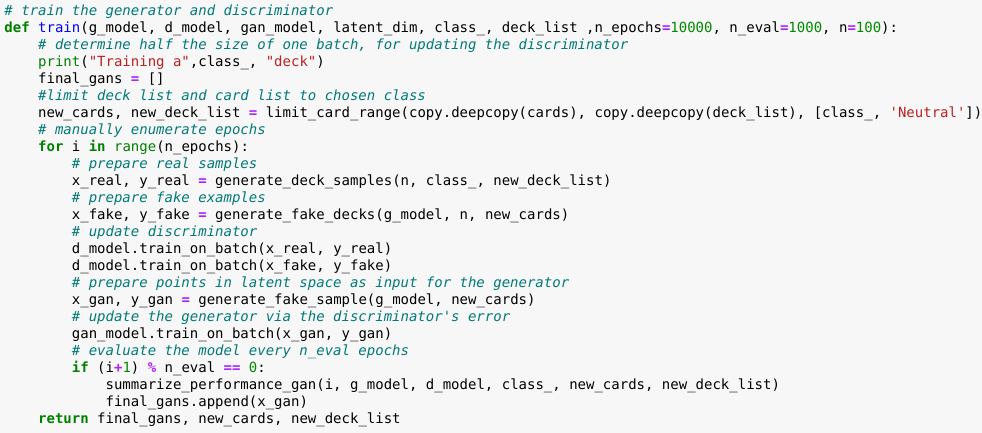
\includegraphics[width=1.25\textwidth]{train}
\caption{Training process of the GAN\protect}
 \label{board}
\end{figure}
\subsubsection{Summarize Performance}
This part of the training process is called every thousand epochs in the training, it is used to evaluate the training process to check the progress, and for any improvements, signs of over-fitting etc...\\ Just like in the training process a real and a fake deck is gathered, however instead of updating the models, instead they are evaluated and a accuracy is return. Since the process is using binary results, the discriminator will evaluate the deck with either a 0 or a 1. Theoretically the discriminator should always display 1 for real decks and then either 0 or 1 for fake ones. After, a graph is drawn displaying the both decks, this is to check their similarity. Refer to figure 5.21 for illustration in code form.

\begin{figure}[H]
\centering
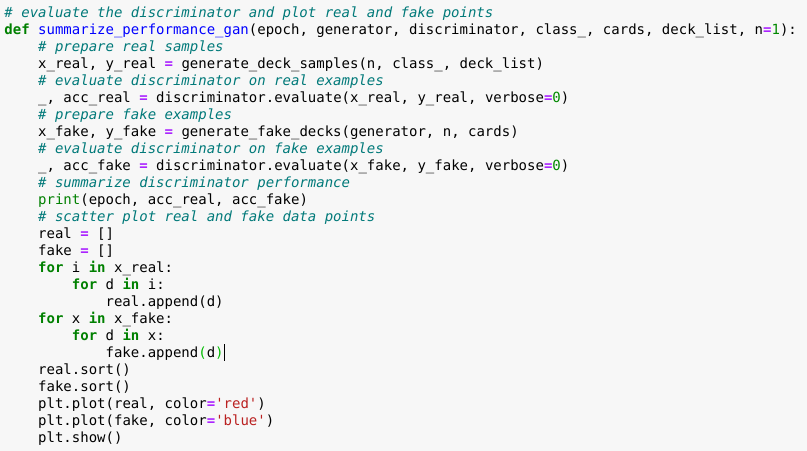
\includegraphics[width=1.25\textwidth]{sumPer}
\caption{Summarize performance of the GAN\protect}
 \label{board}
\end{figure}
\subsection{Initial Results}

Initially the results of the training process were less than ideal, despite having the decks having similar structure (figure 5.22) the issue was that the decks that were created had cards from all the classes. The reason why this happened is because when the GAN trains, it tends to predict cards around the same point as the real cards, but it never produce something identical, and the way the cards are identified is sorted by Hearthstone's default sorting which is cost, so the class cards end up spread across the array of cards the GAN is training from, resulting in multiclass decks that are considered illegal and thus cannot be played. In this case the deck training was limited to the Warrior class dataset, so a method would need to be devised to make a choice.   


\begin{figure}[H]
\centering
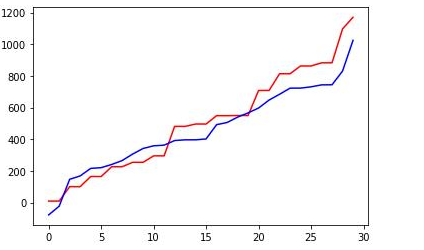
\includegraphics[width=1\textwidth]{initialTraining}
\caption{Similarity between generated and real deck, blue represents fake deck and red the real deck \protect}
 \label{board}
\end{figure}

Another problem that will need to be dealt with is the appearance of negative id's, because of the way the generator model creates decks, some of the cards that are low in the card array can cause the generator to predict negative identifiers for cards, and those cards do not exist. There are a few options that can be considered, such as removing the generated decks that have negative numbers, but will there be any generated decks at the end? The generator model could be changed to not allow negative identifiers to exist, but then there will be a lot of cards of id 0, meaning that there will be more than 2 duplicates of that card resulting in an illegal deck. Or a method that does an absolute of the negative number to make it positive, however if the negative number is too high then it might go outside the range of the card array.\\ \\
Finally, the GAN may not guarantee the generation of legal decks, so a method would need to be written to filter out the illegal decks, such as over 30 cards, more than 2 duplicates of normal cards, duplicates of legendary cards, etc...

\subsection{Improvements}
This section will discuss the improvements that were made to the GAN in order to solve some of the issues discussed previously.
\subsubsection{Class Choice}
The first improvement was to add the ability to select other classes to train a deck for, originally only Warrior decks were trained. A user input was added to allow them to select one of the ten classes to generate a deck. For usability, the user can select by either typing the name of the class or the number it is associated to. This choice is then saved for when the AI training begins, the AI will select the appropriate dataset to train from and will also limit card data to that class, this will be explained in detail in the next section.

\begin{figure}[H]
\centering
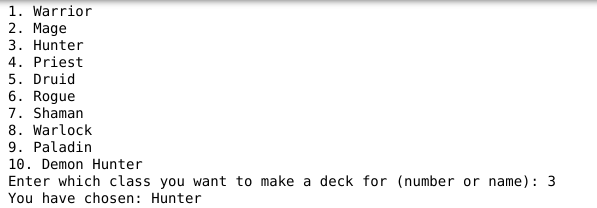
\includegraphics[width=1\textwidth]{choice}
\caption{Choose class results \protect}
 \label{board}
\end{figure}

\subsubsection{Limit Card Data}
Previously, the initial results of the GAN would produce decks with cards from multiple classes, this was a major issue as the GAN did not produce legal decks to play. To fix this, when the user selected a class to create a deck for, the dataset for that class was loaded for training, and the cards were filtered to only have cards of that class and the neutral class, in essence only the cards that the class can use. Once the cards were filtered, the cards identifiers were changed to fit the smaller scale to limit the bounds of the id's, otherwise there could be more predicted id's that do not correspond to cards. Because the card id's were changed, it meant that the id's of the loaded dataset had to be changed aswell. The figure 5.24 below shows the code of this process through the \nolinkurl{limit_card_range} function. 

\begin{figure}[H]
\centering
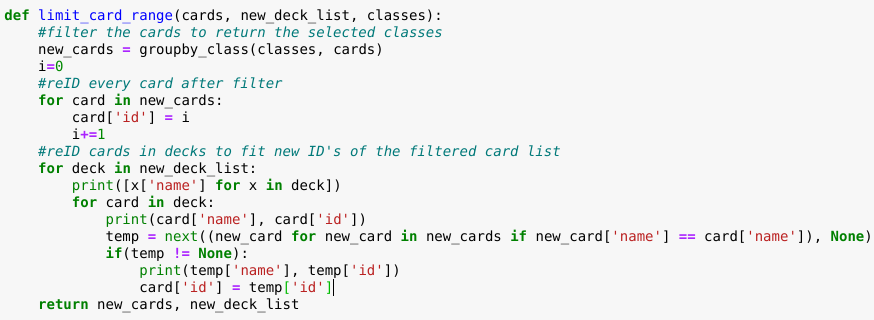
\includegraphics[width=1.25\textwidth]{limitCardRange}
\caption{Limit Range of cards by chosen classes \protect}
 \label{board}
\end{figure}

After this was implemented into the GAN, the resulting decks were legal and showed synergistic card combinations. 

\subsubsection{Deck Verification}

When decks were generated by the AI, it was unclear if the GAN would produced consistently legal decks, for example some decks could have too many duplicates of a card or duplicates of legendaries.

The first check was to convert negative id's to positive ones and check if the converted id's were in legal range of the card list. The second verification needed was see if the created decks had exactly 30 cards. Note that the \nolinkurl{created_gans} array is the array that is returned by the GAN with the generated decks.

\begin{figure}[H]
\centering
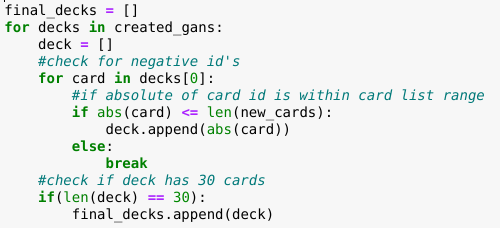
\includegraphics[width=1\textwidth]{abs}
\caption{Convert negative id's and check for legal deck size \protect}
 \label{board}
\end{figure}

Finally, to verify that there are not too many duplicate cards in the deck, a method was written using an array to count the number of instances of a card in a deck. Removing the deck if the duplicates of a card went past 2 for non-legendary cards, and 1 for legendary cards.

\begin{figure}[H]
\centering
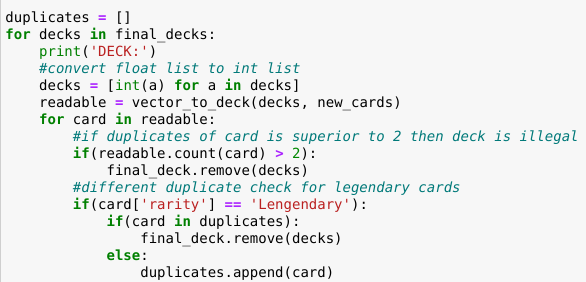
\includegraphics[width=1\textwidth]{duplicates}
\caption{Convert negative id's and check for legal deck size \protect}
 \label{board}
\end{figure}

\chapter{Testing}
\section{Aims}
The aim of the project is to generate playable Hearthstone decks from an AI. The secondary goal is to generate decks with a good win to loss ratio, so more wins than losses. The datasets used for training were collected with a created web scraper, one for each class. To test these decks, a simulator will be used to play the decks, the selection process of the simulator and how it was implemented is explained in the next section.\\
The testing should reflect the following statements: 
\begin{itemize}
\item The overall win rate of a generated deck should be over 50\%, to pertain the relevance of creating a deck
\item A generated deck should have a similar \textbf{type split} to a real deck
\item A generated deck should have a similar \textbf{neutral split} to a real deck
\item A generated deck should have a similar \textbf{mana curve} to a real deck
\item The criteria of a considered legal deck should not be breached, illegal decks should be excluded from the results.
\item The above statements should not be affected by a change of dataset
\end{itemize}
\section{Simulator}
\subsection{Fireplace}
\subsection{Changes}
\subsection{Limitations}
\section{Comparing type split for real and fake decks}
\subsection{Test 1}
\section{Comparing neutral split for real and fake decks}
\section{Comparing mana curve for real and fake decks}
\section{Testing winrates versus Real decks}
\section{Testing winrates versus random decks}

\chapter{Evaluation}
--simulator limited--
%----------------------------------------------------------------------------------------
%	BIBLIOGRAPHY
%---------------------
\bibliography{export}

\chapter{Appendix}
\section*{Appendix A}
\begin{figure}[h]
\centering
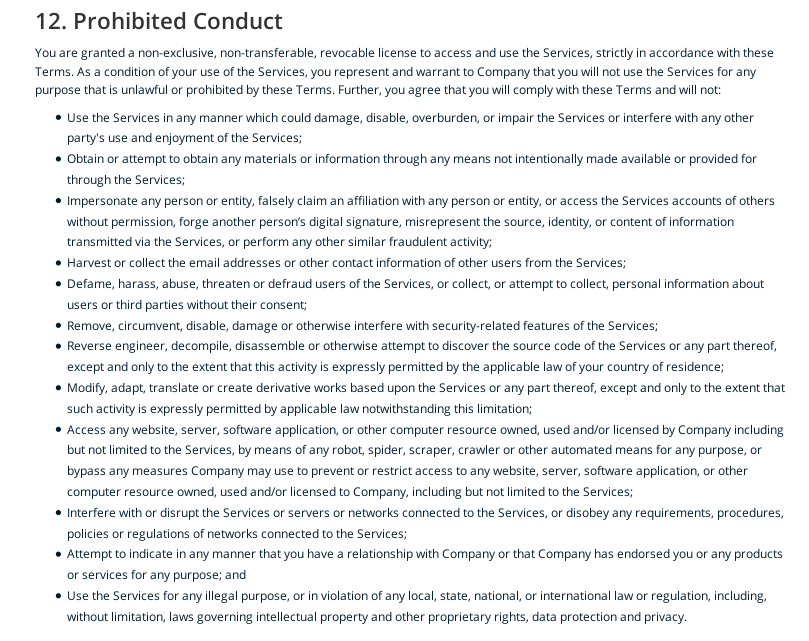
\includegraphics[width=1.25\textwidth]{ProhibitedConduct}
\captionsetup{labelformat=empty}
\caption{Prohibited Conduct section of Hearthpwn Terms of Service\protect}
 \label{board}
\end{figure}
\footnotetext{\url{https://www.magicfind.us/terms/}}


\section*{Appendix B}
\begin{figure}[h]
\centering
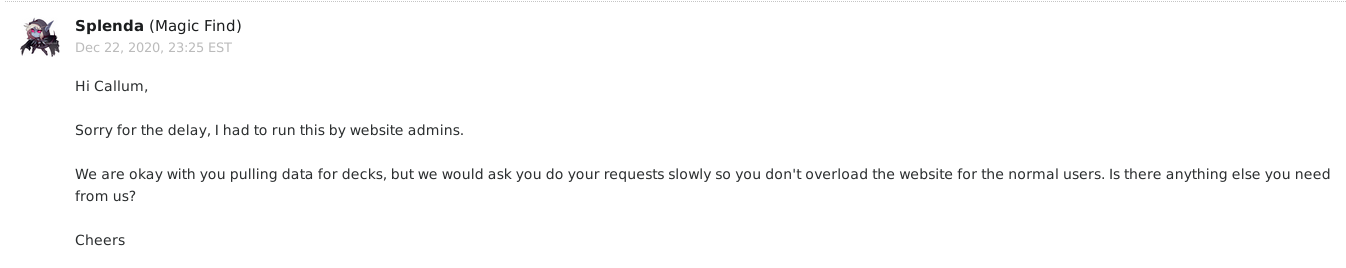
\includegraphics[width=1.25\textwidth]{permission}
\captionsetup{labelformat=empty}
\caption{Permission email from Hearthpwn team\protect\footnotemark}
 \label{board}
\end{figure}

\section*{Appendix C}
\verbatiminput{../../cards-standard-report.txt}

\section*{Appendix D}
\lstinputlisting{../../card-json-example.json}

\section*{Appendix E}
%\begin{figure}[H]
%\centering
%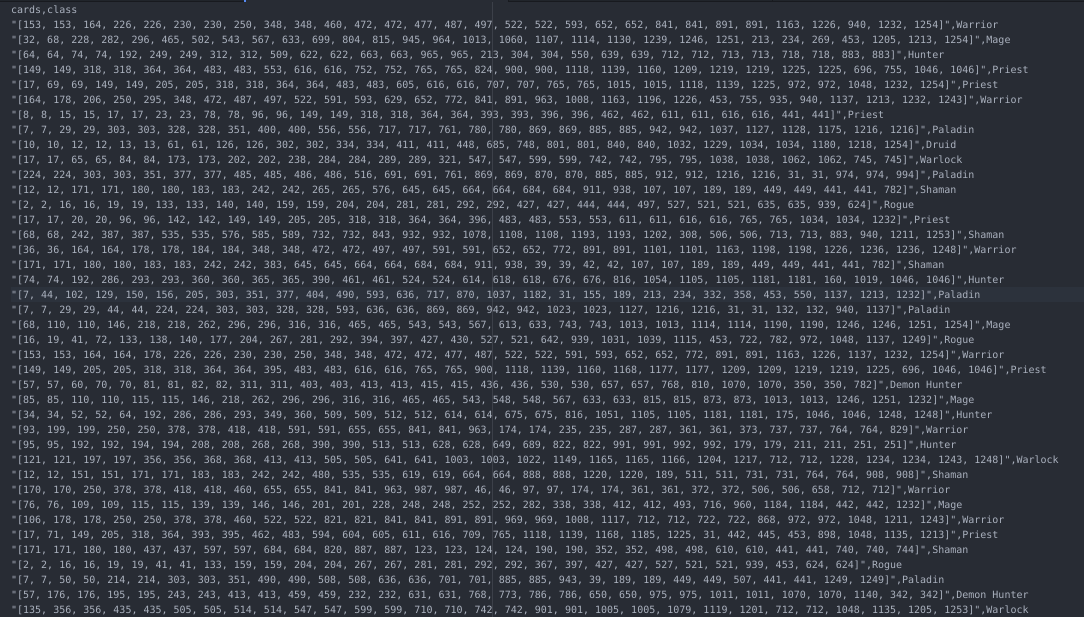
\includegraphics[width=1.25\textwidth]{csv}
% \label{board}
%\end{figure}
\texttt{cards,class\\
"[153, 153, 164, 226, 226, 230, 230, 250, 348, 348, 460, 472, 472, 477, 487, 497, 522, 522, 593, 652, 652, 841, 841, 891, 891, 1163, 1226, 940, 1232, 1254]",Warrior\\
"[32, 68, 228, 282, 296, 465, 502, 543, 567, 633, 699, 804, 815, 945, 964, 1013, 1060, 1107, 1114, 1130, 1239, 1246, 1251, 213, 234, 269, 453, 1205, 1213, 1254]",Mage\\
"[64, 64, 74, 74, 192, 249, 249, 312, 312, 509, 622, 622, 663, 663, 965, 965, 213, 304, 304, 550, 639, 639, 712, 712, 713, 713, 718, 718, 883, 883]",Hunter\\
"[149, 149, 318, 318, 364, 364, 483, 483, 553, 616, 616, 752, 752, 765, 765, 824, 900, 900, 1118, 1139, 1160, 1209, 1219, 1219, 1225, 1225, 696, 755, 1046, 1046]",Priest\\
"[17, 69, 69, 149, 149, 205, 205, 318, 318, 364, 364, 483, 483, 605, 616, 616, 707, 707, 765, 765, 1015, 1015, 1118, 1139, 1225, 972, 972, 1048, 1232, 1254]",Priest\\
"[164, 178, 206, 250, 295, 348, 472, 487, 497, 522, 591, 593, 629, 652, 772, 841, 891, 963, 1008, 1163, 1196, 1226, 453, 755, 935, 940, 1137, 1213, 1232, 1243]",Warrior\\ \\
...\\ \\
"[8, 8, 15, 15, 17, 17, 23, 23, 78, 78, 96, 96, 149, 149, 318, 318, 364, 364, 393, 393, 396, 396, 462, 462, 611, 611, 616, 616, 441, 441]",Priest\\
"[7, 7, 29, 29, 303, 303, 328, 328, 351, 400, 400, 556, 556, 717, 717, 761, 780, 780, 869, 869, 885, 885, 942, 942, 1037, 1127, 1128, 1175, 1216, 1216]",Paladin\\
"[10, 10, 12, 12, 13, 13, 61, 61, 126, 126, 302, 302, 334, 334, 411, 411, 448, 685, 748, 801, 801, 840, 840, 1032, 1229, 1034, 1034, 1180, 1218, 1254]",Druid\\
"[17, 17, 65, 65, 84, 84, 173, 173, 202, 202, 238, 284, 284, 289, 289, 321, 547, 547, 599, 599, 742, 742, 795, 795, 1038, 1038, 1062, 1062, 745, 745]",Warlock\\
"[224, 224, 303, 303, 351, 377, 377, 485, 485, 486, 486, 516, 691, 691, 761, 869, 869, 870, 870, 885, 885, 912, 912, 1216, 1216, 31, 31, 974, 974, 994]",Paladin\\
"[12, 12, 171, 171, 180, 180, 183, 183, 242, 242, 265, 265, 576, 645, 645, 664, 664, 684, 684, 911, 938, 107, 107, 189, 189, 449, 449, 441, 441, 782]",Shaman\\
"[2, 2, 16, 16, 19, 19, 133, 133, 140, 140, 159, 159, 204, 204, 281, 281, 292, 292, 427, 427, 444, 444, 497, 527, 521, 521, 635, 635, 939, 624]",Rogue\\
}

\section*{Appendix F}
\lstinputlisting{../../example-json.json}
%----------------------------------------------------------------------------------------


\end{document}